\chapter{Model validation}
The model was validated comparing the predicted $r_{scc}$ with either behavioural circuit simulations and an experimental circuit.  Because the proposed method has the goal to model losses produced by the charge transfer between capacitors and conductance through resistive elements (switches and parasitics), simulations with a behavioral simulator only take into account these two sources of losses, enabling a fair comparison to validate the proposed model.  Nevertheless, an experimental converter was specifically build with the only propose to measure and validate the model parameters. The converter was designed to mitigate any other source of loss not included in the model, such as switching losses, driving losses, etc. These other loss mechanisms can be added to the model as described in~\cite{Seeman:EECS-2009-78}; however including them is out of the scope of the model presented in the previous chapter.

This chapter is divided in two sections. The first section validates the model for single output SCC using only transient circuit simulations. Results are presented for both output types: The current use, loading the converter at a \emph{dc}-output. and the \emph{hybrid} use, loading the converter at a \emph{pwm}-output.  The second section validates the multiple output model using both circuit simulations and an experimental setup.

\section{Single output validation}
The accuracy of the model is presented for both output types of the converter:
\emph{dc} and \emph{pwm}. In both cases, the validation is performed comparing the predicted $r_{scc}$ values of the model with the measured values from a the behavioural circuit simulator PLECS. In the case of the \emph{dc}-node the results are also compared with the original charge flow analysis, which is the current used methodology.

The same 3:1 Dickson was used as a test circuit. First connecting the load to the \emph{dc}-node as shown in Figure~\ref{fig:3_1_hscc_exp_a}, and second connecting the load to the \emph{pwm}-node as shown in Figure~\ref{fig:3_1_hscc_exp_b}. In both cases the load was emulated with a constant current source. In both simulations the design parameters were kept the same as defied in Table~\ref{tab:sim_values}.

\begin{table}[h]
\centering
\caption{3:1 Dickson design parameters used in PLECS.}
\label{tab:sim_values}
\renewcommand{\arraystretch}{1.5}% Wider
\begin{tabular}{l | c  }
 Parameter  &  Value  \\
 \midrule
 $v_{in}$   & 10V \\
 $r_{on}$   & 100$m\Omega$ \\
 $c_x$      & 100$nF$\\
 $\eta$\footnote{Efficiency} & 95$\%$
\end{tabular}
\end{table}
In order to keep the converter properly operating, the load current $i_{out}$ was adjusted in each simulation by fixing the efficiency to $\eta=95\%$. Hence the load current is given by
\begin{equation}
    i_{out}=m_x~v_{src}\frac{1-\eta}{r_{scc,mdl}},
\label{eq:iout_eff}
\end{equation}
where $m_x$ is the conversion ratio for the given output and $r_{scc,mdl}$ is the predicted output resistance by the model. Fixing the efficiency, guarantees the same average output voltage across all the simulations, since rearranging~\eqref{eq:eff_vo} gives
\begin{equation}
    v_{out}=m_x~v_{src}~\eta.
\label{eq:vout_eff}
\end{equation}
Thus fixing a high efficiency value guarantees that the voltage at the load is close to the target voltage ($v_{trg}=m_x v_{src}$). The load current is small enough to prevent the converter's capacitors from discharging thus avoiding to bring the converter in an undesired operating regime.

\subsection{Measuring $r_{scc}$ from a SCC}
\begin{figure}[!h]
\centering
\ctikzset { bipoles/length=1cm}
\begin{circuitikz}[american,scale=0.65]
\draw
    (2.5,0) to[short]
    (-1.5,0) to[V = $v_{src}$](-1.5,3) -- (2.5,3)
    %(-1.5,3) to[ammeter,l=$i_{in}$]  (1,3) -- (2.5,3)
    (1,3) to[voltmeter,l_=$v_{in}$] (1,0);


\draw [thick]
    (2.5,-0.5) --
    (2.5,3.5)  --
    (5.5,3.5)  --
    (5.5,-0.5) --
    (2.5,-0.5);

\draw (4,1.5) node[align=center]{SCC \\ U.T.} ;

\draw
    (5.5,3) --
    (7,3) to[ammeter,l=$i_{out}$]
    (9.5,3) to[gswitch,l=$s_1$]  (10,3) -- (10.5,3) to[I,l = $i_{load}$]
    (10.5,0) -- (5.5,0)
    (7,3) to[voltmeter,l^=$v_{out}$] (7,0);
\end{circuitikz}
\caption{Experimental arrangement used to measure $r_{scc}$ from a SCC.}
\label{fig:rscc_exp_setup}
\end{figure}
Figure~\ref{fig:rscc_exp_setup} shows the configuration used to measure $r_{scc}$ in the circuit simulator. The $r_{scc}$ is computed measuring the converter in two states, while  keeping constant the driving signals of the converter ($f_{sw}$ and $D$):
\begin{enumerate}
  \item Under no load condition ($s_1$ open). The target voltage $v_{trg}$ and the conversion ration $m$ are determined,
      \begin{align}
        v_{trg} & = v_{out},\label{eq:vtrg}\\
        m & = \frac{v_{out}}{v_{in}}.
        \label{eq:vtrg_m}
      \end{align}

  \item Loading the converter ($s_1$ closed),  $r_{scc}$ is computed using~\eqref{eq:vtrg} as
      \begin{equation}
        r_{scc} = \frac{v_{trg} - v_{out}}{i_{out}}.
        \label{eq:rscc_m}
      \end{equation}
\end{enumerate}

\subsection{ Fixed \emph{dc}-output}
\begin{SCfigure}[][!h]
    \ctikzset { bipoles/length=1cm}
    \centering
    \begin{circuitikz}[american ,scale=0.6]
    \draw
            %Input Supply
            %(0,0)  to[V=$v_{src}$]
            %Draw Switches
            %(0,10)  --
            (5,10.3) node[anchor=south] {$v_{src}$}
            (5,10) node[rground, yscale=-1] {}
            to[gswitch=$s_1$] %S1
            (5,8)   to[gswitch=$s_2$] %S2
            (5,6)   to[gswitch=$s_3$] %S3
            (5,4) --
            %left branch
            (3,4)   to[gswitch=$s_7$]
            (3,2)   to[gswitch=$s_6$]
            (3,0);

    \draw   %right branch
            (5,4) --
            (7,4)   to[gswitch,l_=$s_4$]
            (7,2)   to[gswitch,l_=$s_5$]
            (7,0) -- (3,0);


    \draw %Capacitor C1
           (3,2) -- (2,2) -- (2,4)
            to[pC,l_=$c_1$] (2,8) --
           (5,8);

    \draw %Capacitor C2
           (7,2) --
           (8.25,2) -- (8.25,3.5)  to[pC,l^=$c_2$] (8.25,6) --
           (5,6);

    \draw %Capacitor C3
           (5,0) node[sground] {} to[pC,l_=$c_3$] (5,4);

     %\draw (7,4) to[short,-o] (10,4) node[anchor=west] {};

     %\draw (9,6) to[open,v^=$v_{1}$] (9,0);
     \draw (5,4)  --([hs]8.25,4 |- 5,4) arc(180:0:\radius) to[short] (9.5,4) to[I,l^=$i_{out}$] (9.5,0) |- (5,0);
     \end{circuitikz}
\caption{3:1 Dickson circuit used to validate the model accuracy in the prediction of  $r_{scc}$ for the \emph{dc}-node. Odd numbered switches belong to phase 1, even numbered switches belong to phase 2, and $D$ corresponds to the duty cycle of phase 1.}
\label{fig:3_1_hscc_exp_b}
\end{SCfigure}
Figure~\ref{fig:exp_rscc_dc_node_dx} shows $r_{scc}$ for a sweep in duty cycle ($D$) between $10\%$ and $9\%$, simulated at four different frequencies: 100kHz, 1MHz, 10MHz and 100MHz; thus operating the converter from the SSL to the FSL regions, and in between them. The \emph{$\Box$ markers} are the measured resistance values from the PLECS simulation, the \emph{solid black lines} with \emph{markers}  are the results of the model using the different approximations Original ($\circ$), Markowski ($+$) and modified Markowski($\times$). These different approximations were previously described in Section~\ref{ch:rscc_apprx}. The \emph{grey markers} are the relative error values ($epsilon_r$) between the model results and the PLECS simulation.  The two \emph{gray lines} belong to the results of the previous modeling methods. The \emph{gray dashed line}  corresponds to the results of the original charge flow (OCF) method~\cite{95Makowski} proposed  by~\citeauthor{95Makowski} in~\citeyear{95Makowski}. The dotted line is a posterior addition to the method that includes the effects of the output capacitor, proposed by~\citeauthor{2013Breussegem:c_out} in~\cite{2013Breussegem:c_out}.
\begin{figure}[!h]
\centering
    \begin{subfigure}{\textwidth}
        \parbox[c]{.03\linewidth}{\subcaption{}\label{fig:exp_rscc_dc_node_100kHz}}
        \hspace{.02\linewidth}
        \parbox[c]{.95\linewidth}{
        \centering
        % This file was created by matlab2tikz.
%
%The latest updates can be retrieved from
%  http://www.mathworks.com/matlabcentral/fileexchange/22022-matlab2tikz-matlab2tikz
%where you can also make suggestions and rate matlab2tikz.
%

\begin{tikzpicture}
\pgfplotsset{
    width=9cm,
    height=2.5cm,
    scale only axis,
    xlabel near ticks,
    ylabel near ticks,
    enlarge y limits={0.2},
    legend style={
                legend columns = 3,
                at={(0.5,1.075)},
                anchor=south,
                draw=none,
                font=\small,
                column sep=2ex,
                legend cell align=left},
}

\begin{axis}[%
    axis x line*=bottom,
    axis y line*=left,
    %xlabel= {duty cycle},
    ylabel= {$r_{scc}~[\Omega]$},
    yticklabel style={text width=2em,align=right},
    ]

    \addplot [semithick,mark=square,only marks,white]
      table[y=y1] {./3_modeling/rx_sw_dx_O2.dat};\label{pl_PLECS_hidden}

    \addplot [semithick,mark=square,only marks]
      table[y=y1] {./3_modeling/rx_sw_dx_O2.dat};\label{pl_PLECS}


    \addplot [semithick,smooth,mark=o,mark repeat=10]
      table [y=y1] {./3_modeling/rm1_sw_dx_O2.dat};\label{pl_MDL_JD}

    \addplot [semithick,smooth,mark=+,mark repeat=10]%black!66]
      table [y=y1] {./3_modeling/rm2_sw_dx_O2.dat};\label{pl_Makw}

    \addplot [semithick,smooth,mark=x,mark repeat=10]%black!33]
      table [y=y1] {./3_modeling/rm3_sw_dx_O2.dat};\label{pl_Makw rec}

    \addplot [semithick,smooth,dashed,black!75]
      table [y=y1] {./3_modeling/rm1_ms_sw_dx_O2.dat};\label{pl:95Makw}

    \addplot [semithick,smooth,dotted,black!75]
      table [y=y1] {./3_modeling/rx_ST_sw_dx_1Co.dat};\label{pl:Stey}



\end{axis}

\begin{axis}[%
    axis y line*=right,
    axis x line=none,
    ylabel = {$\epsilon_r~[\%]$},
    yticklabel pos=right,
    yticklabel style={text width=2em,align=left},
    ]
    \addlegendimage{/pgfplots/refstyle=pl_PLECS}\addlegendentry{PLECS}
    \addlegendimage{/pgfplots/refstyle=pl_MDL_JD}\addlegendentry{This Work}

    \addplot [semithick,mark=o,only marks,black!60]
      table [y=y1] {./3_modeling/err1_sw_dx_O2.dat};
    \addlegendentry{ $\epsilon_r$ (Rel. Error)}


    \addlegendimage{/pgfplots/refstyle=pl_PLECS_hidden}\addlegendentry{\color{white}PLECS}
    \addlegendimage{/pgfplots/refstyle=pl_Makw}\addlegendentry{Makowski}
    \addplot [semithick,mark=+,only marks,black!60]
      table [y=y1] {./3_modeling/err2_sw_dx_O2.dat};
    \addlegendentry{$\epsilon_r$ \color{white}(Rel. Error) }

    \addlegendimage{/pgfplots/refstyle=pl_PLECS_hidden}\addlegendentry{\color{white}PLECS}
    \addlegendimage{/pgfplots/refstyle=pl_Makw rec}\addlegendentry{*Mak. }
    \addplot [semithick,mark=x,only marks,black!60]
      table [y=y1] {./3_modeling/err3_sw_dx_O2.dat};
    \addlegendentry{$\epsilon_r$ \color{white}(Rel. Error)}

    \addlegendimage{/pgfplots/refstyle=pl_PLECS_hidden}\addlegendentry{\color{white}PLECS}
    \addlegendimage{/pgfplots/refstyle=pl:95Makw}\addlegendentry{95Makowski.}
    \addlegendimage{/pgfplots/refstyle=pl:Stey}\addlegendentry{Steyaert}


\end{axis}
\end{tikzpicture}




}
    \end{subfigure}

    \begin{subfigure}{\textwidth}
        \parbox[c]{.03\linewidth}{\subcaption{}\label{fig:exp_rscc_dc_node_1MHz}}
        \hspace{.02\linewidth}
        \parbox[c]{.95\linewidth}{
        \centering
        % This file was created by matlab2tikz.
%
%The latest updates can be retrieved from
%  http://www.mathworks.com/matlabcentral/fileexchange/22022-matlab2tikz-matlab2tikz
%where you can also make suggestions and rate matlab2tikz.
%

\begin{tikzpicture}
\pgfplotsset{
    width=9cm,
    height=2.5cm,
    scale only axis,
    ylabel near ticks,
    enlarge y limits={0.2},
    xlabel near ticks,
    ylabel near ticks,
}
\begin{axis}[%
axis x line*=bottom,
axis y line*=left,
xlabel= {duty cycle},
ylabel= {$r_{scc}~[\Omega]$},
yticklabel style={text width=2em,align=right}
]

    \addplot [semithick,mark=square,only marks]
      table[y=y4] {./3_modeling/rx_sw_dx_O2.dat};\label{pl_PLECS}
    \addplot [semithick,smooth,black]
      table [y=y2] {./3_modeling/rm1_sw_dx_O2.dat};\label{pl_MDL}
    \addplot [semithick,smooth,black!66]
      table [y=y2] {./3_modeling/rm2_sw_dx_O2.dat};
    \addplot [semithick,smooth,black!33]
      table [y=y2] {./3_modeling/rm3_sw_dx_O2.dat};
    
    \addplot [semithick,smooth,black,dashed]
      table [y=y2] {./3_modeling/rm1_ms_sw_dx_O2.dat};\label{pl_MDL}

\end{axis}

\begin{axis}[%
    axis y line*=right,
    axis x line=none,
    ylabel = {$\epsilon_r~[\%]$},
    yticklabel pos=right,
    yticklabel style={text width=2em,align=left},
    ]

    \addplot [semithick,mark=star,only marks,black]
    table [y=y4] {./3_modeling/err1_sw_dx_O2.dat};

    \addplot [semithick,mark=star,only marks,black!66]
    table [y=y4] {./3_modeling/err2_sw_dx_O2.dat};

    \addplot [semithick,mark=star,only marks,black!33]
    table [y=y4] {./3_modeling/err3_sw_dx_O2.dat};

\end{axis}
\end{tikzpicture}
}
    \end{subfigure}

    \begin{subfigure}{\textwidth}
        \parbox[c]{.03\linewidth}{\subcaption{}\label{fig:exp_rscc_dc_node_10MHz}}
        \hspace{.02\linewidth}
        \parbox[c]{.95\linewidth}{
        \centering
        % This file was created by matlab2tikz.
%
%The latest updates can be retrieved from
%  http://www.mathworks.com/matlabcentral/fileexchange/22022-matlab2tikz-matlab2tikz
%where you can also make suggestions and rate matlab2tikz.
%

\begin{tikzpicture}
\pgfplotsset{
    width=9cm,
    height=2.5cm,
    scale only axis,
    ylabel near ticks,
    enlarge y limits={0.2},
    xlabel near ticks,
    ylabel near ticks,
}
\begin{axis}[%
axis x line*=bottom,
axis y line*=left,
xlabel= {duty cycle},
ylabel= {$r_{scc}~[\Omega]$},
yticklabel style={text width=2em,align=right},
]

    \addplot [semithick,mark=square,only marks]
      table[y=y7] {./3_modeling/rx_sw_dx_O2.dat};\label{pl_PLECS}
    \addplot [semithick,smooth,black]
      table [y=y3] {./3_modeling/rm1_sw_dx_O2.dat};\label{pl_MDL}
    \addplot [semithick,smooth,black!66]
      table [y=y3] {./3_modeling/rm2_sw_dx_O2.dat};
    \addplot [semithick,smooth,black!33]
      table [y=y3] {./3_modeling/rm3_sw_dx_O2.dat};
    
    \addplot [semithick,smooth,black,dashed]
      table [y=y3] {./3_modeling/rm1_ms_sw_dx_O2.dat};\label{pl_MDL}

\end{axis}

\begin{axis}[%
axis y line*=right,
axis x line=none,
ylabel = {$\epsilon_r~[\%]$},
yticklabel pos=right,
yticklabel style={text width=2em,align=left},
]

    \addplot [semithick,mark=star,only marks,black]
    table [y=y7] {./3_modeling/err1_sw_dx_O2.dat};

    \addplot [semithick,mark=star,only marks,black!66]
    table [y=y7] {./3_modeling/err2_sw_dx_O2.dat};

    \addplot [semithick,mark=star,only marks,black!33]
    table [y=y7] {./3_modeling/err3_sw_dx_O2.dat};

\end{axis}
\end{tikzpicture}
}
    \end{subfigure}

    \begin{subfigure}{\textwidth}
        \parbox[c]{.03\linewidth}{\subcaption{}\label{fig:exp_rscc_dc_node_100MHz}}
        \hspace{.02\linewidth}
        \parbox[c]{.95\linewidth}{
        \centering
        % This file was created by matlab2tikz.
%
%The latest updates can be retrieved from
%  http://www.mathworks.com/matlabcentral/fileexchange/22022-matlab2tikz-matlab2tikz
%where you can also make suggestions and rate matlab2tikz.
%

\begin{tikzpicture}
\pgfplotsset{
    width=9cm,
    height=2.5cm,
    scale only axis,
    ylabel near ticks,
    enlarge y limits={0.2},
    xlabel near ticks,
    ylabel near ticks,
}
\begin{axis}[%
axis x line*=bottom,
axis y line*=left,
xlabel= {duty cycle},
ylabel= {$r_{scc}~[\Omega]$},
yticklabel style={text width=2em,align=right},
]

\addplot [semithick,mark=square,only marks,forget plot]
  table {./3_modeling/sim_rx_100MHz_O2.dat};

\addplot [semithick,solid,forget plot]
  table {./3_modeling/mdl_rx_100MHz_O2.dat};

%\addplot [semithick,dashed,forget plot]
%  table {./3_modeling/mdl_see_rx_100MHz_O1.dat};

\end{axis}

\begin{axis}[%
axis y line*=right,
axis x line=none,
ylabel = {$\epsilon_r~[\%]$},
yticklabel pos=right,
yticklabel style={text width=2em,align=left},
]

\addplot [semithick,mark=star,only marks,forget plot]
  table {./3_modeling/error_rx_100MHz_O2.dat};


\end{axis}
\end{tikzpicture}
}
    \end{subfigure}

\caption{$r_{scc}$ from the \emph{dc}-node of the converter of Figure~\ref{fig:3_1_hscc_exp_b}. \emph{$\Box$ markers} are the experimental results compared with the \emph{solid black lines} predicted by the model at different $f_{sw}$ \emph{top-to-bottom}: $100kHz$, $1MHz$, $10MHz$ and $100MHz$. The model results are given for the different approximations: Original ($\circ$), Makowski ($+$), Makowski modified ($\times$); and the \emph{gray markers} are the relative error for the different approximations. The \emph{dashed gray line} corresponds to the original charge flow analysis, and the \emph{dotted gray line} to a posterior enhancement including the effects of the output capacitor.}
\label{fig:exp_rscc_dc_node_dx}
\end{figure}

\begin{figure}[!h]
\newcommand\pHeigh{3.25cm}
\newcommand\pWidth{2.5cm}
\centering
    \begin{subfigure}{\textwidth}
       \parbox[b]{.325\linewidth}{
            \raggedright
            % This file was created by matlab2tikz.
%
%The latest updates can be retrieved from
%  http://www.mathworks.com/matlabcentral/fileexchange/22022-matlab2tikz-matlab2tikz
%where you can also make suggestions and rate matlab2tikz.
%

\begin{tikzpicture}
\pgfplotsset{
    width=\pWidth,
    height=\pHeigh,
    scale only axis,
    ylabel near ticks,
    enlarge y limits={0.2},
    xlabel near ticks,
    ylabel near ticks,
    enlarge x limits={0.15},
    every tick label/.append style={font=\footnotesize},
}

\begin{loglogaxis}[
		axis y line*=left,
        axis x line*=bottom,
        xticklabels={,,},
        enlarge y limits={0.1},
        ytick = {1e1,1},
        ylabel= {$ r_{scc} ~ [\Omega] $} ,
        %yticklabel style={xshift=0.5ex},
        title={$c_o= c_{fly}$},
        title style = {
                at ={(0.5,1.1)} },
        legend style={
                legend columns = -1,
                at={(0.5,0.97)},
                anchor=south,
                draw=none,
                font=\tiny,
                column sep=1ex},
        ]


    \addplot [thin,mark=square,only marks,black]
      table [y=y1]{./3_modeling/rx_sw_fsw_1Co.dat};
    \addplot [thin,smooth,black,mark=o,mark repeat=2]
      table [y=y1]{./3_modeling/rx_JD_sw_fsw_1Co.dat};\label{pl_MDL}
    %\addlegendentry{Model};
    \addplot [thin,smooth,mark=+,mark repeat=2]
      table [y=y1]{./3_modeling/rx_MS_sw_fsw_1Co.dat};
    %\addlegendentry{Seeman};
    \addplot [thin,smooth,mark=x,mark repeat=2]
      table [y=y1]{./3_modeling/rx_ST_sw_fsw_1Co.dat};
    %\addlegendentry{Steyaert};


\end{loglogaxis}

\begin{semilogxaxis}[%
    axis y line*=right,
    axis x line=none,
    %ylabel = {$\epsilon_r~[\%]$},
    yticklabel pos=right,
    yticklabel style={text width=1em,align=left,xshift=-0.5ex},
    enlarge y limits={0.25},
    legend style={
                    legend columns = -1,
                    at={(0.5,0.95)},
                    anchor=south,
                    draw=none,
                    font=\tiny,
                    column sep=1ex},
    ]


    \addplot [semithick,mark=o,only marks,black!50]
      table [y=y1]{./3_modeling/err_JD_sw_fsw_1Co.dat};
    \addplot [semithick,mark=+,only marks,black!50]
      table [y=y1]{./3_modeling/err_MS_sw_fsw_1Co.dat};
    \addplot [semithick,mark=x,only marks,black!50]
      table [y=y1]{./3_modeling/err_ST_sw_fsw_1Co.dat};

\end{semilogxaxis}

\end{tikzpicture}

        }
       \parbox[b]{.325\linewidth}{
            \raggedleft
            % This file was created by matlab2tikz.
%
%The latest updates can be retrieved from
%  http://www.mathworks.com/matlabcentral/fileexchange/22022-matlab2tikz-matlab2tikz
%where you can also make suggestions and rate matlab2tikz.
%

\begin{tikzpicture}
\pgfplotsset{
    width=\pWidth,
    height=\pHeigh,
    scale only axis,
    ylabel near ticks,
    enlarge y limits={0.2},
    xlabel near ticks,
    ylabel near ticks,
    enlarge x limits={0.15},
    every tick label/.append style={font=\footnotesize},
}
\begin{loglogaxis}[
        xticklabels={,,},
        axis y line*=left,
        axis x line*=bottom,
        ytick = {1e1,1},
        enlarge y limits={0.1},
        yticklabel style={text width=3em,align=right,xshift=0.5ex},
        title={$c_o= 10 c_{fly}$},
        title style = {
                at ={(0.5,1.2)} },
        ]

    \addplot [thin,mark=square,only marks,white]
      table [y=y1]{./3_modeling/rx_sw_fsw_10Co.dat};\label{pl_PLECS_hid}

    \addplot [thin,mark=square,only marks,black]
      table [y=y1]{./3_modeling/rx_sw_fsw_10Co.dat};\label{pl_PLECS}

    \addplot [thin,smooth,black,mark=o,mark repeat=2]
      table [y=y1]{./3_modeling/rx_JD_sw_fsw_10Co.dat};\label{pl_MDL}
    %\addlegendentry{Model};
    \addplot [thin,smooth,mark=+,mark repeat=2]
      table [y=y1]{./3_modeling/rx_MS_sw_fsw_10Co.dat};\label{pl_MS}
    %\addlegendentry{Seeman};
    \addplot [thin,smooth,mark=x,mark repeat=2]
      table [y=y1]{./3_modeling/rx_ST_sw_fsw_10Co.dat};\label{pl_ST}
    %\addlegendentry{Steyaert};


\end{loglogaxis}

\begin{semilogxaxis}[%
    axis y line*=right,
    axis x line=none,
    yticklabel pos=right,
    yticklabel style={text width=1em,align=left,xshift=-0.5ex},
    enlarge y limits={0.25},
    legend style={
                    legend columns = 3,
                    at={(0.5,0.95)},
                    anchor=south,
                    draw=none,
                    font=\tiny,
                    column sep=0.5ex},
    ]

    \addlegendimage{/pgfplots/refstyle=pl_PLECS}\addlegendentry{PLECS}
    \addlegendimage{/pgfplots/refstyle=pl_MDL}\addlegendentry{This work}
    \addplot [semithick,mark=o,only marks,black!50]
      table [y=y1]{./3_modeling/err_JD_sw_fsw_10Co.dat};
    \addlegendentry{ $\epsilon_r$}

    \addlegendimage{/pgfplots/refstyle=pl_PLECS_hid}\addlegendentry{\color{white}PLECS}
    \addlegendimage{/pgfplots/refstyle=pl_MS}\addlegendentry{OCF}
    \addplot [semithick,mark=+,only marks,black!50]
      table [y=y1]{./3_modeling/err_MS_sw_fsw_10Co.dat};
    \addlegendentry{ $\epsilon_r$}

    \addlegendimage{/pgfplots/refstyle=pl_PLECS_hid}\addlegendentry{\color{white}PLECS}
    \addlegendimage{/pgfplots/refstyle=pl_ST}\addlegendentry{Steyaert}
    \addplot [semithick,mark=x,only marks,black!50]
      table [y=y1]{./3_modeling/err_ST_sw_fsw_10Co.dat};
    \addlegendentry{ $\epsilon_r$}

\end{semilogxaxis}

\end{tikzpicture}

        }
       \parbox[b]{.325\linewidth}{
            \centering
            % This file was created by matlab2tikz.
%
%The latest updates can be retrieved from
%  http://www.mathworks.com/matlabcentral/fileexchange/22022-matlab2tikz-matlab2tikz
%where you can also make suggestions and rate matlab2tikz.
%

\begin{tikzpicture}
\pgfplotsset{
    width=\pWidth,
    height=\pHeigh,
    scale only axis,
    ylabel near ticks,
    enlarge y limits={0.2},
    xlabel near ticks,
    ylabel near ticks,
    enlarge x limits={0.15},
}
\begin{loglogaxis}[
        %xlabel= {$f_{sw}[Hz] $},
        xticklabels={,,},
        %ylabel= {$ r_{scc} ~ [\Omega] $} ,
        axis y line*=left,
        axis x line*=bottom,
        ytick = {1e1,1},
        %xtick=\empty, ytick=\empty,
        %ytick = {0,.125,.25},
        %yticklabels={0,$v_{src}\frac{1}{3}$,$v_{src}\frac{2}{3}$,$v_{src}$},
        %xticklabels={0,$D \cdot T_{sw}$,$T_{sw}$ ,$2 T_{sw}$,$3 T_{sw} $},
        enlarge y limits={0.1},
        yticklabel style={text width=2em,align=right},
        title={$c_o= 100 c_{fly}$},
        title style = {
                at ={(0.5,1.1)} },
        legend style={
                legend columns = -1,
                at={(0.5,0.95)},
                anchor=south,
                draw=none,
                font=\tiny,
                column sep=1ex},
        ]

    \addplot [thin,mark=square,only marks,black]
      table [y=y1]{./3_modeling/rx_sw_fsw_100Co.dat};
    \addplot [thin,smooth,black,mark=o,mark repeat=2]
      table [y=y1]{./3_modeling/rx_JD_sw_fsw_100Co.dat};\label{pl_MDL}
    %\addlegendentry{Model};
    \addplot [thin,smooth,mark=+,mark repeat=2]
      table [y=y1]{./3_modeling/rx_MS_sw_fsw_100Co.dat};
    %\addlegendentry{Seeman};
    \addplot [thin,smooth,mark=x,mark repeat=2]
      table [y=y1]{./3_modeling/rx_ST_sw_fsw_100Co.dat};
    %\addlegendentry{Steyaert};


\end{loglogaxis}

\begin{semilogxaxis}[%
    axis y line*=right,
    axis x line=none,
    ylabel = {$\epsilon_r~[\%]$},
    yticklabel pos=right,
    yticklabel style={text width=2em,align=left},
    enlarge y limits={0.25},
    legend style={
                    legend columns = -1,
                    at={(0.5,0.95)},
                    anchor=south,
                    draw=none,
                    font=\tiny,
                    column sep=1ex},
    ]


    \addplot [semithick,mark=o,only marks,black!60]
      table [y=y1]{./3_modeling/err_JD_sw_fsw_100Co.dat};
    \addplot [semithick,mark=+,only marks,black!50]
      table [y=y1]{./3_modeling/err_MS_sw_fsw_100Co.dat};
    \addplot [semithick,mark=x,only marks,black!50]
      table [y=y1]{./3_modeling/err_ST_sw_fsw_100Co.dat};

\end{semilogxaxis}

\end{tikzpicture}

        }
    \end{subfigure}

    \begin{subfigure}{\textwidth}
       \parbox[b]{.325\linewidth}{
            \raggedright
            % This file was created by matlab2tikz.
%
%The latest updates can be retrieved from
%  http://www.mathworks.com/matlabcentral/fileexchange/22022-matlab2tikz-matlab2tikz
%where you can also make suggestions and rate matlab2tikz.
%

\begin{tikzpicture}
\pgfplotsset{
    width=\pWidth,
    height=\pHeigh,
    scale only axis,
    ylabel near ticks,
    enlarge y limits={0.2},
    xlabel near ticks,
    ylabel near ticks,
    enlarge x limits={0.15},
    every tick label/.append style={font=\footnotesize},
}

\begin{loglogaxis}[
        %xlabel= {$f_{sw}[Hz] $},
        xticklabels={,,},
        ylabel= {$ r_{scc} ~ [\Omega] $} ,
        axis y line*=left,
        axis x line*=bottom,
        ytick = {1e1,1},
        yticklabel style={xshift=0.5ex},
        enlarge y limits={0.1},
        domain=10e6:10e8,
        legend style={
                legend columns = -1,
                at={(0.5,0.95)},
                anchor=south,
                draw=none,
                font=\tiny,
                column sep=1ex},
        ]

    \addplot [thin,mark=square,only marks,black]
      table [y=y2]{./3_modeling/rx_sw_fsw_1Co.dat};
    \addplot [thin,smooth,black,mark=o,mark repeat=2]
      table [y=y2]{./3_modeling/rx_JD_sw_fsw_1Co.dat};\label{pl_MDL}
    %\addlegendentry{Model};
    \addplot [thin,smooth,mark=+,mark repeat=2]
      table [y=y2]{./3_modeling/rx_MS_sw_fsw_1Co.dat};
    %\addlegendentry{Seeman};
    \addplot [thin,smooth,mark=x,mark repeat=2]
      table [y=y2]{./3_modeling/rx_ST_sw_fsw_1Co.dat};
    %\addlegendentry{Steyaert};


\end{loglogaxis}

\begin{semilogxaxis}[%
    axis y line*=right,
    axis x line=none,
    %ylabel = {$\epsilon_r~[\%]$},
    yticklabel pos=right,
    yticklabel style={text width=2em,align=left},
    enlarge y limits={0.25},
    legend style={
                    legend columns = -1,
                    at={(0.5,0.95)},
                    anchor=south,
                    draw=none,
                    font=\tiny,
                    column sep=1ex},
    ]


    \addplot [semithick,mark=o,only marks,black!50]
      table [y=y2]{./3_modeling/err_JD_sw_fsw_1Co.dat};
    \addplot [semithick,mark=+,only marks,black!50]
      table [y=y2]{./3_modeling/err_MS_sw_fsw_1Co.dat};
    \addplot [semithick,mark=x,only marks,black!50]
      table [y=y2]{./3_modeling/err_ST_sw_fsw_1Co.dat};

\end{semilogxaxis}
\end{tikzpicture}

        }
       \parbox[b]{.325\linewidth}{
            \raggedleft
            % This file was created by matlab2tikz.
%
%The latest updates can be retrieved from
%  http://www.mathworks.com/matlabcentral/fileexchange/22022-matlab2tikz-matlab2tikz
%where you can also make suggestions and rate matlab2tikz.
%

\begin{tikzpicture}
\pgfplotsset{
    width=\pWidth,
    height=\pHeigh,
    scale only axis,
    ylabel near ticks,
    enlarge y limits={0.2},
    xlabel near ticks,
    ylabel near ticks,
    enlarge x limits={0.15},
    every tick label/.append style={font=\footnotesize},
}

\begin{loglogaxis}[
        %xlabel= {$f_{sw}[Hz] $},
        xticklabels={,,},
        %ylabel= {$ r_{scc} ~ [\Omega] $} ,
        axis y line*=left,
        axis x line*=bottom,
        ytick = {1e1,1},
        %xticklabels = {$10^1$,,4,8},
        %xtick=\empty, ytick=\empty,
        %ytick = {0,.125,.25},
        %yticklabels={0,$v_{src}\frac{1}{3}$,$v_{src}\frac{2}{3}$,$v_{src}$},
        %xticklabels={0,$D \cdot T_{sw}$,$T_{sw}$ ,$2 T_{sw}$,$3 T_{sw} $},
        enlarge y limits={0.1},
        yticklabel style={text width=3em,align=right,xshift=0.5ex},
        %title={$c_o= 10 c_{fly}$},
        legend style={
                legend columns = -1,
                at={(0.5,0.95)},
                anchor=south,
                draw=none,
                font=\tiny,
                column sep=1ex},
        ]

    \addplot [thin,mark=square,only marks,black]
      table [y=y2]{./3_modeling/rx_sw_fsw_10Co.dat};
    \addplot [thin,smooth,black,mark=o,mark repeat=2]
      table [y=y2]{./3_modeling/rx_JD_sw_fsw_10Co.dat};\label{pl_MDL}
    %\addlegendentry{Model};
    \addplot [thin,smooth,mark=+,mark repeat=2]
      table [y=y2]{./3_modeling/rx_MS_sw_fsw_10Co.dat};
    %\addlegendentry{Seeman};
    \addplot [thin,smooth,mark=x,mark repeat=2]
      table [y=y2]{./3_modeling/rx_ST_sw_fsw_10Co.dat};
    %\addlegendentry{Steyaert};


\end{loglogaxis}

\begin{semilogxaxis}[%
    axis y line*=right,
    axis x line=none,
    %ylabel = {$\epsilon_r~[\%]$},
    yticklabel pos=right,
    yticklabel style={text width=2em,align=left,xshift=-0.5ex},
    enlarge y limits={0.25},
    legend style={
                    legend columns = -1,
                    at={(0.5,0.95)},
                    anchor=south,
                    draw=none,
                    font=\tiny,
                    column sep=1ex},
    ]


    \addplot [semithick,mark=o,only marks,black!50]
      table [y=y2]{./3_modeling/err_JD_sw_fsw_10Co.dat};
    \addplot [semithick,mark=+,only marks,black!50]
      table [y=y2]{./3_modeling/err_MS_sw_fsw_10Co.dat};
    \addplot [semithick,mark=x,only marks,black!50]
      table [y=y2]{./3_modeling/err_ST_sw_fsw_10Co.dat};

\end{semilogxaxis}

\end{tikzpicture}

        }
       \parbox[b]{.325\linewidth}{
            \centering
            % This file was created by matlab2tikz.
%
%The latest updates can be retrieved from
%  http://www.mathworks.com/matlabcentral/fileexchange/22022-matlab2tikz-matlab2tikz
%where you can also make suggestions and rate matlab2tikz.
%

\begin{tikzpicture}
\pgfplotsset{
    width=\pWidth,
    height=\pHeigh,
    scale only axis,
    ylabel near ticks,
    enlarge y limits={0.2},
    xlabel near ticks,
    ylabel near ticks,
    enlarge x limits={0.15},
}

\begin{loglogaxis}[
        %xlabel= {$f_{sw}[Hz] $},
        xticklabels={,,},
        %ylabel= {$ r_{scc} ~ [\Omega] $} ,
        axis y line*=left,
        axis x line*=bottom,
        ytick = {1e1,1},
        %xtick=\empty, ytick=\empty,
        %ytick = {0,.125,.25},
        %yticklabels={0,$v_{src}\frac{1}{3}$,$v_{src}\frac{2}{3}$,$v_{src}$},
        %xticklabels={0,$D \cdot T_{sw}$,$T_{sw}$ ,$2 T_{sw}$,$3 T_{sw} $},
        enlarge y limits={0.1},
        yticklabel style={text width=2em,align=right},
        %title={$c_o= 10 c_{fly}$},
        legend style={
                legend columns = -1,
                at={(0.5,0.95)},
                anchor=south,
                draw=none,
                font=\tiny,
                column sep=1ex},
        ]

    \addplot [thin,mark=square,only marks,black]
      table [y=y2]{./3_modeling/rx_sw_fsw_100Co.dat};
    \addplot [thin,smooth,black,mark=o,mark repeat=2]
      table [y=y2]{./3_modeling/rx_JD_sw_fsw_100Co.dat};\label{pl_MDL}
    %\addlegendentry{Model};
    \addplot [thin,smooth,mark=+,mark repeat=2]
      table [y=y2]{./3_modeling/rx_MS_sw_fsw_100Co.dat};
    %\addlegendentry{Seeman};
    \addplot [thin,smooth,mark=x,mark repeat=2]
      table [y=y2]{./3_modeling/rx_ST_sw_fsw_100Co.dat};
    %\addlegendentry{Steyaert};


\end{loglogaxis}

\begin{semilogxaxis}[%
    axis y line*=right,
    axis x line=none,
    ylabel = {$\epsilon_r~[\%]$},
    yticklabel pos=right,
    yticklabel style={text width=2em,align=left},
    enlarge y limits={0.25},
    legend style={
                    legend columns = -1,
                    at={(0.5,0.95)},
                    anchor=south,
                    draw=none,
                    font=\tiny,
                    column sep=1ex},
    ]


    \addplot [semithick,mark=o,only marks,black!60]
      table [y=y2]{./3_modeling/err_JD_sw_fsw_100Co.dat};
    \addplot [semithick,mark=+,only marks,black!50]
      table [y=y2]{./3_modeling/err_MS_sw_fsw_100Co.dat};
    \addplot [semithick,mark=x,only marks,black!50]
      table [y=y2]{./3_modeling/err_ST_sw_fsw_100Co.dat};

\end{semilogxaxis}

\end{tikzpicture}

        }
    \end{subfigure}

    \begin{subfigure}{\textwidth}
       \parbox[b]{.325\linewidth}{
            \raggedright
            % This file was created by matlab2tikz.
%
%The latest updates can be retrieved from
%  http://www.mathworks.com/matlabcentral/fileexchange/22022-matlab2tikz-matlab2tikz
%where you can also make suggestions and rate matlab2tikz.
%

\begin{tikzpicture}
\pgfplotsset{
    width=\pWidth,
    height=\pHeigh,
    scale only axis,
    ylabel near ticks,
    enlarge y limits={0.2},
    xlabel near ticks,
    ylabel near ticks,
    enlarge x limits={0.15},
    every tick label/.append style={font=\footnotesize},
}

\begin{loglogaxis}[
        xlabel= {$f_{sw}[Hz] $},
        ylabel= {$ r_{scc} ~ [\Omega] $} ,
        axis y line*=left,
        axis x line*=bottom,
        ytick = {1e1,1},
        yticklabel style={xshift=0.5ex},
        enlarge y limits={0.2},
        legend style={
                legend columns = -1,
                at={(0.5,0.95)},
                anchor=south,
                draw=none,
                font=\tiny,
                column sep=1ex},
        ]



    \addplot [thin,mark=square,only marks,black]
      table [y=y3]{./3_modeling/rx_sw_fsw_1Co.dat};
    \addplot [thin,smooth,black,mark=o,mark repeat=2]
      table [y=y3]{./3_modeling/rx_JD_sw_fsw_1Co.dat};\label{pl_MDL}
    %\addlegendentry{Model};
    \addplot [thin,smooth,mark=+,mark repeat=2]
      table [y=y3]{./3_modeling/rx_MS_sw_fsw_1Co.dat};
    %\addlegendentry{Seeman};
    \addplot [thin,smooth,mark=x,mark repeat=2]
      table [y=y3]{./3_modeling/rx_ST_sw_fsw_1Co.dat};
    %\addlegendentry{Steyaert};


\end{loglogaxis}

\begin{semilogxaxis}[%
    axis y line*=right,
    axis x line=none,
    %ylabel = {$\epsilon_r~[\%]$},
    yticklabel pos=right,
    yticklabel style={text width=2em,align=left},
    enlarge y limits={0.25},
    legend style={
                    legend columns = -1,
                    at={(0.5,0.95)},
                    anchor=south,
                    draw=none,
                    font=\tiny,
                    column sep=1ex},
    ]


    \addplot [semithick,mark=o,only marks,black!60]
      table [y=y3]{./3_modeling/err_JD_sw_fsw_1Co.dat};
    \addplot [semithick,mark=+,only marks,black!50]
      table [y=y3]{./3_modeling/err_MS_sw_fsw_1Co.dat};
    \addplot [semithick,mark=x,only marks,black!50]
      table [y=y3]{./3_modeling/err_ST_sw_fsw_1Co.dat};

\end{semilogxaxis}
\end{tikzpicture}

        }
       \parbox[b]{.325\linewidth}{
            \raggedleft
            % This file was created by matlab2tikz.
%
%The latest updates can be retrieved from
%  http://www.mathworks.com/matlabcentral/fileexchange/22022-matlab2tikz-matlab2tikz
%where you can also make suggestions and rate matlab2tikz.
%

\begin{tikzpicture}
\pgfplotsset{
    width=\pWidth,
    height=\pHeigh,
    scale only axis,
    ylabel near ticks,
    enlarge y limits={0.2},
    xlabel near ticks,
    ylabel near ticks,
    enlarge x limits={0.15},
    every tick label/.append style={font=\footnotesize},
}

\begin{loglogaxis}[
        xlabel= {$f_{sw}[Hz] $},
        axis y line*=left,
        axis x line*=bottom,
        ytick = {1e1,1},
        enlarge y limits={0.1},
        yticklabel style={text width=3em,align=right,xshift=0.5ex},
        legend style={
                legend columns = -1,
                at={(0.5,0.95)},
                anchor=south,
                draw=none,
                font=\tiny,
                column sep=1ex},
        ]

    \addplot [thin,mark=square,only marks,black]
      table [y=y3]{./3_modeling/rx_sw_fsw_10Co.dat};
    \addplot [thin,smooth,black,mark=o,mark repeat=2]
      table [y=y3]{./3_modeling/rx_JD_sw_fsw_10Co.dat};\label{pl_MDL}
    %\addlegendentry{Model};
    \addplot [thin,smooth,mark=+,mark repeat=2]
      table [y=y3]{./3_modeling/rx_MS_sw_fsw_10Co.dat};
    %\addlegendentry{Seeman};
    \addplot [thin,smooth,mark=x,mark repeat=2]
      table [y=y3]{./3_modeling/rx_ST_sw_fsw_10Co.dat};
    %\addlegendentry{Steyaert};


\end{loglogaxis}

\begin{semilogxaxis}[%
    axis y line*=right,
    axis x line=none,
    %ylabel = {$\epsilon_r~[\%]$},
    yticklabel pos=right,
    yticklabel style={text width=2em,align=left,xshift=-0.5ex},
    enlarge y limits={0.25},
    legend style={
                    legend columns = -1,
                    at={(0.5,0.95)},
                    anchor=south,
                    draw=none,
                    font=\tiny,
                    column sep=1ex},
    ]


    \addplot [semithick,mark=o,only marks,black!50]
      table [y=y3]{./3_modeling/err_JD_sw_fsw_10Co.dat};
    \addplot [semithick,mark=+,only marks,black!50]
      table [y=y3]{./3_modeling/err_MS_sw_fsw_10Co.dat};
    \addplot [semithick,mark=x,only marks,black!50]
      table [y=y3]{./3_modeling/err_ST_sw_fsw_10Co.dat};

\end{semilogxaxis}


\end{tikzpicture}

        }
       \parbox[b]{.325\linewidth}{
            \centering
            % This file was created by matlab2tikz.
%
%The latest updates can be retrieved from
%  http://www.mathworks.com/matlabcentral/fileexchange/22022-matlab2tikz-matlab2tikz
%where you can also make suggestions and rate matlab2tikz.
%

\begin{tikzpicture}
\pgfplotsset{
    width=\pWidth,
    height=\pHeigh,
    scale only axis,
    ylabel near ticks,
    enlarge y limits={0.2},
    xlabel near ticks,
    ylabel near ticks,
    enlarge x limits={0.15},
    every tick label/.append style={font=\footnotesize},
}


\begin{loglogaxis}[
        xlabel= {$f_{sw}[Hz] $},
        %xticklabels={,,},
        %ylabel= {$ r_{scc} ~ [\Omega] $} ,
        axis y line*=left,
        axis x line*=bottom,
        ytick = {1e1,1},
        enlarge y limits={0.1},
        yticklabel style={text width=2em,align=right,xshift=0.5ex},
        %title={$c_o= 10 c_{fly}$},
        legend style={
                legend columns = -1,
                at={(0.5,0.95)},
                anchor=south,
                draw=none,
                font=\tiny,
                column sep=1ex},
        ]

    \addplot [thin,mark=square,only marks,black]
      table [y=y3]{./3_modeling/rx_sw_fsw_100Co.dat};
    \addplot [thin,smooth,black,mark=o,mark repeat=2]
      table [y=y3]{./3_modeling/rx_JD_sw_fsw_100Co.dat};\label{pl_MDL}
    %\addlegendentry{Model};
    \addplot [thin,smooth,mark=+,mark repeat=2]
      table [y=y3]{./3_modeling/rx_MS_sw_fsw_100Co.dat};
    %\addlegendentry{Seeman};
    \addplot [thin,smooth,mark=x,mark repeat=2]
      table [y=y3]{./3_modeling/rx_ST_sw_fsw_100Co.dat};
    %\addlegendentry{Steyaert};


\end{loglogaxis}

\begin{semilogxaxis}[%
    axis y line*=right,
    axis x line=none,
    ylabel = {$\epsilon_r~[\%]$},
    yticklabel pos=right,
    yticklabel style={text width=2em,align=left,xshift=-0.5ex},
    enlarge y limits={0.25},
    legend style={
                    legend columns = -1,
                    at={(0.5,0.95)},
                    anchor=south,
                    draw=none,
                    font=\tiny,
                    column sep=1ex},
    ]


    \addplot [semithick,mark=o,only marks,black!50]
      table [y=y3]{./3_modeling/err_JD_sw_fsw_100Co.dat};
    \addplot [semithick,mark=+,only marks,black!50]
      table [y=y3]{./3_modeling/err_MS_sw_fsw_100Co.dat};
    \addplot [semithick,mark=x,only marks,black!50]
      table [y=y3]{./3_modeling/err_ST_sw_fsw_100Co.dat};

\end{semilogxaxis}

\end{tikzpicture}

        }
    \end{subfigure}



\caption{$r_{scc}$ from the \emph{dc}-node of the converter of Figure~\ref{fig:3_1_hscc_exp_b} for a sweep of $f_{sw}$. \emph{$\Box$ markers} are the experimental points. The \emph{solid black lines} are the different modeling methods, and the \emph{gray markers} the relative error of each method. Plots are presented for different duty cycles:  \emph{Rows top-to-bottom}- $D = 23.3\%$, $D = 50\%$ and $D = 76.7\%$. And also for different $c_o$ values: \emph{columns left-to-right}- $c_{fly}$ , $10~c_{fly} $ and $100~c_{cfly}$.}
\label{fig:exp_rscc_dc_node}
\end{figure}

Looking to the relative error  of the model with respect to the PLECS simulation, it can be seen that on the one hand the two extreme simulations Figures~\ref{fig:exp_rscc_dc_node_100kHz} and~\ref{fig:exp_rscc_dc_node_100MHz} achieve the highest accuracy with a relative error $\epsilon_r$ lower than $1\%$ at $100kHz$ and $4\%$ at $100MHz$. In this two simulations the converter operates in the well-defined switching limits, SSL and FSL, therefore the losses are precisely described by the model.  On the other hand, the other two simulations, $1MHz$ and $10MHz$,  have an error within $5\%$ to $20\%$. The accuracy is reduced since the converter operates between of two switching limits, hence $r_{scc}$ is approximated from the two asymptotical functions. Looking to the different approximation methods (\emph{gray markers}), we can see that the original approximation for $r_{scc}$ presents the best accuracy in all the simulations. Independently of the model accuracy, it can be seen that predictive trends (in all fourth plots of Figure~\ref{fig:exp_rscc_dc_node_dx}) are still consistent for variations in duty cycle.

The plotted results of the current methods (\emph{gray lines}) make evident their  limitations in the prediction of $r_{scc}$. Actually , these limitations come from modeling the load as a voltage sink, as described in Section~\ref{ch:load_model}, which neglects the effects of the duty cycle ($D$) and the output capacitor ($c_o$) in the prediction of $r_{ssl}$. Figures~\ref{fig:exp_rscc_dc_node_100kHz} and~\ref{fig:exp_rscc_dc_node_1MHz} show the converter operating in the SSL region. The original charge flow  method \emph{OCF} (\emph{gray dashed line}) only matches the measured value in PLECS when the duty cycle is close to $20\%$ and overestimates its value for the majority of the range. Steyaert proposed a modification of the charge flow method that takes into account the output capacitor in the prediction of $r_{ssc}$, however the predicted $r_{scc}$ (\emph{gray dotted line}) does not show a better trend than the original method. In this case, $r_{scc}$ presents a lower value, only matching the measured value for $D=65\%$. Indeed, both plots make evident that predicted $r_{scc}$ is independent to the duty cycle, which is not the case for the new proposed methodology (\emph{solid curves}).  When the converter operates in the FSL region, there are no differences between the methods as it can be seen in Figure~\ref{fig:exp_rscc_dc_node_1MHz}.

\begin{figure}[!h]
\newcommand\pHeigh{3.25cm}
\newcommand\pWidth{4cm}
\centering
    \begin{subfigure}{\textwidth}
       \parbox[b]{.45\linewidth}{
            \raggedright
            % This file was created by matlab2tikz.
%
%The latest updates can be retrieved from
%  http://www.mathworks.com/matlabcentral/fileexchange/22022-matlab2tikz-matlab2tikz
%where you can also make suggestions and rate matlab2tikz.
%

\begin{tikzpicture}
\pgfplotsset{
    width=\pWidth,
    height=\pHeigh,
    scale only axis,
    ylabel near ticks,
    enlarge y limits={0.2},
    xlabel near ticks,
    ylabel near ticks,
    enlarge x limits={0.15},
    every tick label/.append style={font=\footnotesize},
}

\begin{loglogaxis}[
		axis y line*=left,
        axis x line*=bottom,
        %xticklabels={,,},
        enlarge y limits={0.1},
        ytick = {1e1,1},
        ylabel= {$ r_{scc} ~ [\Omega] $},
        xlabel = {$f_{sw}~[Hz]$},
        %yticklabel style={xshift=0.5ex},
        title={$c_o= c_{fly}$},
        title style = {
                at ={(0.5,1.1)} },
        legend style={
                legend columns = -1,
                at={(0.5,0.97)},
                anchor=south,
                draw=none,
                font=\tiny,
                column sep=1ex},
        ]

    \addplot [thin,smooth,black,mark=o,mark repeat=2,gray]
      table [y=y1]{./3_modeling/rx_MS_sw_fsw_1Co.dat};\label{pl_MDL}

    \addplot [thin,smooth,black,mark=+,mark repeat=2,gray]
      table [y=y2]{./3_modeling/rx_MS_sw_fsw_1Co.dat};\label{pl_MDL}

    \addplot [thin,smooth,black,mark=x,mark repeat=2,gray]
      table [y=y3]{./3_modeling/rx_MS_sw_fsw_1Co.dat};\label{pl_MDL}
    
    \addplot [thin,smooth,black,mark=o,mark repeat=2]
      table [y=y1]{./3_modeling/rx_JD_sw_fsw_1Co.dat};\label{pl_MDL}
    
    \addplot [thin,smooth,black,mark=+,mark repeat=2]
      table [y=y2]{./3_modeling/rx_JD_sw_fsw_1Co.dat};\label{pl_MDL}
    
    \addplot [thin,smooth,black,mark=x,mark repeat=2]
      table [y=y3]{./3_modeling/rx_JD_sw_fsw_1Co.dat};\label{pl_MDL}
    


\end{loglogaxis}


\end{tikzpicture}

        }
       \parbox[b]{.45\linewidth}{
            \raggedleft
            % This file was created by matlab2tikz.
%
%The latest updates can be retrieved from
%  http://www.mathworks.com/matlabcentral/fileexchange/22022-matlab2tikz-matlab2tikz
%where you can also make suggestions and rate matlab2tikz.
%

\begin{tikzpicture}
\pgfplotsset{
    width=\pWidth,
    height=\pHeigh,
    scale only axis,
    ylabel near ticks,
    enlarge y limits={0.2},
    xlabel near ticks,
    ylabel near ticks,
    enlarge x limits={0.15},
    every tick label/.append style={font=\footnotesize},
}

\begin{loglogaxis}[
		axis y line*=left,
        axis x line*=bottom,
        %xticklabels={,,},
        enlarge y limits={0.1},
        ytick = {1e1,1},
        %ylabel= {$ r_{scc} ~ [\Omega] $} ,
        xlabel = {$f_{sw}~[Hz]$},
        %yticklabel style={xshift=0.5ex},
        title={$c_o= 10c_{fly}$},
        title style = {
                at ={(0.5,1.1)} },
        legend style={
                legend columns = -1,
                at={(0.5,0.97)},
                anchor=south,
                draw=none,
                font=\tiny,
                column sep=1ex},
        ]


     \addplot [thin,smooth,black,mark=o,mark repeat=2,gray]
      table [y=y1]{./3_modeling/rx_MS_sw_fsw_10Co.dat};\label{pl_MDL}

    \addplot [thin,smooth,black,mark=+,mark repeat=2,gray]
      table [y=y2]{./3_modeling/rx_MS_sw_fsw_10Co.dat};\label{pl_MDL}

    \addplot [thin,smooth,black,mark=x,mark repeat=2,gray]
      table [y=y3]{./3_modeling/rx_MS_sw_fsw_10Co.dat};\label{pl_MDL}

    \addplot [thin,smooth,black,mark=o,mark repeat=2]
      table [y=y1]{./3_modeling/rx_JD_sw_fsw_10Co.dat};\label{pl_MDL}

    \addplot [thin,smooth,black,mark=+,mark repeat=2]
      table [y=y2]{./3_modeling/rx_JD_sw_fsw_10Co.dat};\label{pl_MDL}

    \addplot [thin,smooth,black,mark=x,mark repeat=2]
      table [y=y3]{./3_modeling/rx_JD_sw_fsw_10Co.dat};\label{pl_MDL}

\end{loglogaxis}


\end{tikzpicture}

        }
    \end{subfigure}
\end{figure}



The other limitation of the original method is that it leads to inaccuracies when the output capacitor $c_o$ becomes comparable in value to the rest of the capacitors in the converter. The plots in Figure~\ref{fig:exp_rscc_dc_node} present $r_{scc}$ for a sweep in frequency. In the figure, each row is associated to a duty cycle, hence in the top row $D=23.3\%$, middle $D=50\%$ and bottom $D=76.7\%$. Each column is associated to a different size of the output capacitor $c_o$, hence left column $c_o=c_{fly}$, middle $c_o=10c_{fly}$, and right $c_o=100c_{fly}$, being $c_{fly}=c_1=c_2 =100nF$. The square markers present the measured values of $r_{scc}$ using PLECS, the \emph{solid black lines} present the three modeling methods, and the \emph{grey markers} are $\epsilon_r$ with respect to the PLECS results.

Reading the plots from left to right, it can be seen that for the two old methods (\emph{$+$ and $\times$ markers}) the relative error reduces as $c_o$ increases, achieving a almost the same accuracy of the new proposed method for largest value of $c_o$. Looking in detail, we observe that the highest inaccuracies are in the SSL region, in the low frequency range. At the same time, between the two old methodologies, the original methodology has a higher accuracy for $D=23.3\%$, and in the other cases Steyaert's modification achieves an smaller error. Actually, in the original charge flow method it was assumed $D=50\%$ when operating in the SSL region, therefore Steyaert's modification would be, under this assumption, better. In any case, the results show clearly that the best accuracy is achieved with the new proposed methodology, keeping the relative error within the same limits for all different scenarios. We can observe in all plots the lowest accuracy is around the elbow of the $r_{scc}$ curve, since the values are approximated from the two asymptotical limits.

\begin{figure}[!h]
\newcommand\pHeigh{5cm}
\newcommand\pWidth{7cm}
\centering
     % This file was created by matlab2tikz.
%
%The latest updates can be retrieved from
%  http://www.mathworks.com/matlabcentral/fileexchange/22022-matlab2tikz-matlab2tikz
%where you can also make suggestions and rate matlab2tikz.
%

\begin{tikzpicture}
\pgfplotsset{
    width=\pWidth,
    height=\pHeigh,
    scale only axis,
    xlabel near ticks,
    ylabel near ticks,
    enlarge x limits={0.15},
    enlarge y limits={0.2},
}

\begin{semilogxaxis}[
        xlabel= {$c_{out}/c_{fly} $},
        %xticklabels={,,},
        ylabel= {$ r_{scc} ~ [\Omega] $} ,
        axis y line*=left,
        axis x line*=bottom,
        ymax= 24,
        ymin= 0,
        domain = 0.15:50,
        %xticklabels = {$10^1$,,4,8},
        %xtick=\empty, ytick=\empty,
        %ytick = {0,.125,.25},
        %yticklabels={0,$v_{src}\frac{1}{3}$,$v_{src}\frac{2}{3}$,$v_{src}$},
        %xticklabels={0,$D \cdot T_{sw}$,$T_{sw}$ ,$2 T_{sw}$,$3 T_{sw} $},
        enlarge y limits={0.1},
        yticklabel style={text width=2em,align=right},
        %title={$c_o= 10 c_{fly}$},
        legend style={
                legend columns = 2,
                at={(0.5,0.95)},
                anchor=south,
                draw=none,
                font=\small,
                column sep=1ex},
        ]


    \addplot [thin,mark=square,black,only marks]
      table [y=y1]{./3_modeling/r_scc_sweep_Cout_100kHz_dc.dat};
      \addlegendentry{PLECS};
    \addplot [thick,smooth,black]
      table [y=y1]{./3_modeling/rx_JD_sw_Cout_fsw100k.dat};
      \addlegendentry{This Work};
    \addplot [thick,smooth,dashed]
      table [y=y1]{./3_modeling/rx_MS_sw_Cout_fsw100k.dat};
      \addlegendentry{Makowski};
    \addplot [thick,smooth,dotted]
      table [y=y1]{./3_modeling/rx_ST_sw_Cout_fsw100k.dat};
      \addlegendentry{Steyaert};

\end{semilogxaxis}

\end{tikzpicture}

     \caption{Equivalent Output Resistance ($r_{scc}$) as function of the relative size of the output capacitor (\emph{dc}-capacitor) with respect to the flying capacitors for the 3:1 Dickson converter of Figure~\ref{fig:3_1_hscc_exp_b}. Results presented for the converter operating at $f_{sw}=100kHz$ with capacitors $c_1=c_2=c_{fly}=100nF$ and all switch resistances $r_{on} = 100m\Omega$.}\label{fig:exp_rscc_pwm_node_fsw}
\end{figure}

The influence of $c_o$ in $r_{scc}$ can be better visualized in the plot of  Figure~\ref{fig:exp_rscc_pwm_node_fsw}. The results are given for the converter operating with $D=50\%$, the \emph{$\Box$ markers} are the measured values of $r_{scc}$, and the solid lines the different modeling methodologies. We can see that as the output capacitor reduces, $r_{scc}$ reduces as well till a certain minimum point where it starts increasing again. From the three modeling methodologies, only the  proposed in this work follows the measured data. Actually the reason for the decrease of the output resistance value is because a smaller output capacitor allows the other capacitors to contribute in delivering charge to the load. However reducing the output capacitor increases the voltage ripple at the output node. In~\cite{14Andersen} are exploited the advantages of reducing the output capacitor in order to increase the power density in a full integrated SCC.
%\clearpage
\subsection{ Floating \emph{pwm}-output }
Figures~\ref{fig:exp_rscc_pwm_node_dx} and~\ref{fig:exp_rscc_pwm_node_fsw} present the results of $r_{scc}$ for a sweep of the duty cycle ($D$) and frequency ($f_{sw}$) respectively. In both figures, the results are presented using the different approximations described in Section~\ref{ch:rscc_apprx}.

\begin{SCfigure}[][!h]
    \ctikzset { bipoles/length=1cm}
    \centering
    \begin{circuitikz}[american,scale=0.6]
    \draw
            %Input Supply
            %(0,0)  to[V=$v_{src}$]
            %Draw Switches
            %(0,10)  --
            (5,10.3) node[anchor=south] {$v_{src}$}
            (5,10) node[rground, yscale=-1] {}
            to[gswitch=$s_1$] %S1
            (5,8)   to[gswitch=$s_2$] %S2
            (5,6)   to[gswitch=$s_3$] %S3
            (5,4) --
            %left branch
            (3,4)   to[gswitch=$s_7$]
            (3,2)   to[gswitch=$s_6$]
            (3,0);

    \draw   %right branch
            (5,4) --
            (7,4)   to[gswitch,l_=$s_4$]
            (7,2)   to[gswitch,l_=$s_5$]
            (7,0) -- (3,0);


    \draw %Capacitor C1
           (3,2) -- (2,2) -- (2,4)
            to[pC,l_=$c_1$] (2,8) --
           (5,8);

    \draw %Capacitor C2
           (7,2) --
           (8.25,2) -- (8.25,3.5)  to[pC,l^=$c_2$] (8.25,6) --
           (5,6);

    \draw %Capacitor C3
           (5,0) node[sground] {} to[pC,l_=$c_3$] (5,4);

     %\draw (7,4) to[short,-o] (10,4) node[anchor=west] {};

     %\draw (9,6) to[open,v^=$v_{1}$] (9,0);
     %\draw (8.25,6) to[short,-o] (9,6) node[anchor=west] {$v_{out}$} ;
     \draw (8.25,6) -- (9.5,6) to[I,l^=$i_{out}$] (9.5,0) |- (5,0);
     \end{circuitikz}
\caption{3:1 H$^2$-Dickson circuit used to validate the model accuracy in the prediction of  $r_{scc}$ for the \emph{pwm}-node. Odd numbered switches belong to phase 1, even numbered switches belong to phase 2, and $D$ corresponds to the duty cycle of phase 1.}
\label{fig:3_1_hscc_exp_a}
\end{SCfigure}

Figure~\ref{fig:exp_rscc_pwm_node_dx} presents a sweep in duty cycle for different frequencies, respectively: $100kHz$, $1MHz$, $10MHz$ and $100MHz$. Like in the results for the \emph{dc}-node, the two extreme cases, top and bottom, present the highest accuracy with $\epsilon_r$ below the $2\%$, since the converter operate in the deep regions of the two well-defined operation limits: SSL (Figure~\ref{fig:exp_rscc_pwm_node_100kHz}) and FSL (Figure~\ref{fig:exp_rscc_pwm_node_100MHz}). Outside the deep operation limits (Figures~\ref{fig:exp_rscc_pwm_node_1MHz} and~\ref{fig:exp_rscc_pwm_node_10MHz}), the accuracy is decreased, being  up to an order of magnitude higher, since the values are approximated from the two asymptotic limits. Regarding to the different approximation methods, again the original formulation ( $r_{scc} = \sqrt{r_{ssl}^2 + r_{fsl}^2}$ ) achieves the best results.

Figure~\ref{fig:exp_rscc_pwm_node_fsw} presents $r_{scc}$ for a sweep of the switching frequency $f_{sw}$, showing the well-known characteristic curve of $r_{scc}$. Results are presented  for different duty cycles. Consistent with the previous results, the accuracy is always reduced in the elbow of the curve where the converter operates in between the two limiting regions. At the same time, extreme duty cycles show smaller relative error ($\epsilon_r$). However this smaller values in $\epsilon_r$ are also influenced by the higher values of $r_{scc}$ at these regions.  Looking to the different approximations of $r_{scc}$, as in the previous case, the original formulation still obtains the best accuracy. Independently of the model accuracy, it can be seen that predictive trends, in all presented results, are still consistent for variations in duty cycle and frequency.

\begin{figure}[!h]
\centering
    \begin{subfigure}{\textwidth}
        \parbox[c]{.03\linewidth}{\subcaption{}\label{fig:exp_rscc_pwm_node_100kHz}}
        \hspace{.02\linewidth}
        \parbox[c]{.95\linewidth}{
        \centering
        % This file was created by matlab2tikz.
%
%The latest updates can be retrieved from
%  http://www.mathworks.com/matlabcentral/fileexchange/22022-matlab2tikz-matlab2tikz
%where you can also make suggestions and rate matlab2tikz.
%

\begin{tikzpicture}
\pgfplotsset{
    width=9cm,
    height=2.5cm,
    scale only axis,
    xlabel near ticks,
    ylabel near ticks,
    enlarge y limits={0.2},
    legend style={
                legend columns = 3,
                at={(0.5,1.075)},
                anchor=south,
                draw=none,
                font=\small,
                column sep=2ex,
                legend cell align=left},
}

\begin{axis}[%
    axis x line*=bottom,
    axis y line*=left,
    %xlabel= {duty cycle},
    ylabel= {$r_{scc}~[\Omega]$},
    yticklabel style={text width=2em,align=right},
    ]
    
    \addplot [semithick,mark=square,only marks,white]
      table[y=y1] {./3_modeling/rx_sw_dx_O1.dat};\label{pl_PLECS_hidden}

    \addplot [semithick,mark=square,only marks]
      table[y=y1] {./3_modeling/rx_sw_dx_O1.dat};\label{pl_PLECS}


    \addplot [semithick,smooth,mark=o,mark repeat=10]
      table [y=y1] {./3_modeling/rm1_sw_dx_O1.dat};\label{pl_MDL_JD}

    \addplot [semithick,smooth,mark=+,mark repeat=10]%black!66]
      table [y=y1] {./3_modeling/rm2_sw_dx_O1.dat};\label{pl_Makw}

    \addplot [semithick,smooth,mark=x,mark repeat=10]%black!33]
      table [y=y1] {./3_modeling/rm3_sw_dx_O1.dat};\label{pl_Makw rec}



\end{axis}

\begin{axis}[%
    axis y line*=right,
    axis x line=none,
    ylabel = {$\epsilon_r~[\%]$},
    yticklabel pos=right,
    yticklabel style={text width=2em,align=left},
    ]
    \addlegendimage{/pgfplots/refstyle=pl_PLECS}\addlegendentry{PLECS}
    \addlegendimage{/pgfplots/refstyle=pl_MDL_JD}\addlegendentry{This Work}

    \addplot [semithick,mark=o,only marks,black!60]
      table [y=y1] {./3_modeling/err1_sw_dx_O1.dat};
    \addlegendentry{ $\epsilon_r$ (Rel. Error)}


    \addlegendimage{/pgfplots/refstyle=pl_PLECS_hidden}\addlegendentry{\color{white}PLECS}
    \addlegendimage{/pgfplots/refstyle=pl_Makw}\addlegendentry{Makowski}
    \addplot [semithick,mark=+,only marks,black!60]
      table [y=y1] {./3_modeling/err2_sw_dx_O1.dat};
    \addlegendentry{$\epsilon_r$ \color{white}(Rel. Error) }

    \addlegendimage{/pgfplots/refstyle=pl_PLECS_hidden}\addlegendentry{\color{white}PLECS}
    \addlegendimage{/pgfplots/refstyle=pl_Makw rec}\addlegendentry{Mak. rect.}
    \addplot [semithick,mark=x,only marks,black!60]
      table [y=y1] {./3_modeling/err3_sw_dx_O1.dat};
    \addlegendentry{$\epsilon_r$ \color{white}(Rel. Error)}

\end{axis}
\end{tikzpicture}




}
    \end{subfigure}

    \begin{subfigure}{\textwidth}
        \parbox[c]{.03\linewidth}{\subcaption{}\label{fig:exp_rscc_pwm_node_1MHz}}
        \hspace{.02\linewidth}
        \parbox[c]{.95\linewidth}{
        \centering
        % This file was created by matlab2tikz.
%
%The latest updates can be retrieved from
%  http://www.mathworks.com/matlabcentral/fileexchange/22022-matlab2tikz-matlab2tikz
%where you can also make suggestions and rate matlab2tikz.
%

\begin{tikzpicture}
\pgfplotsset{
    width=9cm,
    height=2.5cm,
    scale only axis,
    ylabel near ticks,
    enlarge y limits={0.2},
    xlabel near ticks,
    ylabel near ticks,
}
\begin{axis}[%
axis x line*=bottom,
axis y line*=left,
xlabel= {duty cycle},
ylabel= {$r_{scc}~[\Omega]$},
yticklabel style={text width=2em,align=right}
]

    \addplot [semithick,mark=square,only marks]
      table[y=y4] {./3_modeling/rx_sw_dx_O1.dat};\label{pl_PLECS}
    \addplot [semithick,smooth,black]
      table [y=y2] {./3_modeling/rm1_sw_dx_O1.dat};\label{pl_MDL}
    \addplot [semithick,smooth,black!66]
      table [y=y2] {./3_modeling/rm2_sw_dx_O1.dat};
    \addplot [semithick,smooth,black!33]
      table [y=y2] {./3_modeling/rm3_sw_dx_O1.dat};

\end{axis}

\begin{axis}[%
    axis y line*=right,
    axis x line=none,
    ylabel = {$\epsilon_r~[\%]$},
    yticklabel pos=right,
    yticklabel style={text width=2em,align=left},
    ]

    \addplot [semithick,mark=star,only marks,black]
    table [y=y4] {./3_modeling/err1_sw_dx_O1.dat};
          
    \addplot [semithick,mark=star,only marks,black!66]
    table [y=y4] {./3_modeling/err2_sw_dx_O1.dat};

    \addplot [semithick,mark=star,only marks,black!33]
    table [y=y4] {./3_modeling/err3_sw_dx_O1.dat};

\end{axis}
\end{tikzpicture}
}
    \end{subfigure}

    \begin{subfigure}{\textwidth}
        \parbox[c]{.03\linewidth}{\subcaption{}\label{fig:exp_rscc_pwm_node_10MHz}}
        \hspace{.02\linewidth}
        \parbox[c]{.95\linewidth}{
        \centering
        % This file was created by matlab2tikz.
%
%The latest updates can be retrieved from
%  http://www.mathworks.com/matlabcentral/fileexchange/22022-matlab2tikz-matlab2tikz
%where you can also make suggestions and rate matlab2tikz.
%

\begin{tikzpicture}
\pgfplotsset{
    width=9cm,
    height=2.5cm,
    scale only axis,
    ylabel near ticks,
    enlarge y limits={0.2},
    xlabel near ticks,
    ylabel near ticks,
}
\begin{axis}[%
axis x line*=bottom,
axis y line*=left,
%xlabel= {duty cycle},
ylabel= {$r_{scc}~[\Omega]$},
yticklabel style={text width=2em,align=right},
]

    \addplot [semithick,mark=square,only marks]
      table[y=y7] {./3_modeling/rx_sw_dx_O1.dat};\label{pl_PLECS}
    \addplot [semithick,smooth,mark=o,mark repeat=10]
      table [y=y3] {./3_modeling/rm1_sw_dx_O1.dat};\label{pl_MDL_JD}
    \addplot [semithick,smooth,mark=+,mark repeat=10]%black!66]
      table [y=y3] {./3_modeling/rm2_sw_dx_O1.dat};\label{pl_Makw}
    \addplot [semithick,smooth,mark=x,mark repeat=10]%black!33]
      table [y=y3] {./3_modeling/rm3_sw_dx_O1.dat};\label{pl_Makw rec}

\end{axis}

\begin{axis}[%
axis y line*=right,
axis x line=none,
ylabel = {$\epsilon_r~[\%]$},
yticklabel pos=right,
yticklabel style={text width=2em,align=left},
]

    \addplot [semithick,mark=o,only marks,black!60]
    table [y=y7] {./3_modeling/err1_sw_dx_O1.dat};

    \addplot [semithick,mark=+,only marks,black!60]
    table [y=y7] {./3_modeling/err2_sw_dx_O1.dat};

    \addplot [semithick,mark=x,only marks,black!60]
    table [y=y7] {./3_modeling/err3_sw_dx_O1.dat};

\end{axis}
\end{tikzpicture}
}
    \end{subfigure}

    \begin{subfigure}{\textwidth}
        \parbox[c]{.03\linewidth}{\subcaption{}\label{fig:exp_rscc_pwm_node_100MHz}}
        \hspace{.02\linewidth}
        \parbox[c]{.95\linewidth}{
        \centering
        % This file was created by matlab2tikz.
%
%The latest updates can be retrieved from
%  http://www.mathworks.com/matlabcentral/fileexchange/22022-matlab2tikz-matlab2tikz
%where you can also make suggestions and rate matlab2tikz.
%

\begin{tikzpicture}
\pgfplotsset{
    width=9cm,
    height=2.5cm,
    scale only axis,
    ylabel near ticks,
    enlarge y limits={0.2},
    xlabel near ticks,
    ylabel near ticks,
}
\begin{axis}[%
axis x line*=bottom,
axis y line*=left,
xlabel= {duty cycle},
ylabel= {$r_{scc}~[\Omega]$},
yticklabel style={text width=2em,align=right},
]

\addplot [semithick,mark=square,only marks,forget plot]
  table {./3_modeling/sim_rx_100MHz_O1.dat};

\addplot [semithick,solid,forget plot]
  table {./3_modeling/mdl_rx_100MHz_O1.dat};

\end{axis}

\begin{axis}[%
axis y line*=right,
axis x line=none,
ylabel = {$\epsilon_r~[\%]$},
yticklabel pos=right,
yticklabel style={text width=2em,align=left},
]

\addplot [semithick,mark=star,only marks,forget plot]
  table {./3_modeling/error_rx_100MHz_O1.dat};


\end{axis}
\end{tikzpicture}
}
    \end{subfigure}

\caption{$r_{scc}$ from the \emph{pwm}-node of the converter of Figure~\ref{fig:3_1_hscc_exp_b}. \emph{$\Box$ markers} are the experimental results compared with the \emph{solid black lines} predicted by the model at different $f_{sw}$ \emph{top-to-bottom}: $100kHz$, $1MHz$, $10MHz$ and $100MHz$. The model results are given for the different approximations: Original ($\circ$), Makowski ($+$), Makowski modified ($\times$); and the \emph{gray markers} are the relative error for the different approximations.  }
\label{fig:exp_rscc_pwm_node_dx}
\end{figure}

\begin{figure}[!h]
\centering
    \begin{subfigure}{0.45\textwidth}
        % This file was created by matlab2tikz.
%
%The latest updates can be retrieved from
%  http://www.mathworks.com/matlabcentral/fileexchange/22022-matlab2tikz-matlab2tikz
%where you can also make suggestions and rate matlab2tikz.
%

\begin{tikzpicture}
\pgfplotsset{
    width=4.5cm,
    height=3.25cm,
    scale only axis,
    ylabel near ticks,
    enlarge y limits={0.2},
    xlabel near ticks,
    ylabel near ticks,
    enlarge x limits={0.15},
}
\begin{loglogaxis}[
        %xlabel= {$f_{sw}[Hz] $},
        xticklabels={,,},
        ylabel= {$ r_{scc} ~ [\Omega] $} ,
        axis y line*=left,
        axis x line*=bottom,
        %xtick=\empty, ytick=\empty,
        %ytick = {0,.125,.25},
        %yticklabels={0,$v_{src}\frac{1}{3}$,$v_{src}\frac{2}{3}$,$v_{src}$},
        %xticklabels={0,$D \cdot T_{sw}$,$T_{sw}$ ,$2 T_{sw}$,$3 T_{sw} $},
        enlarge y limits={0.2},
        title={$D=10\%$},
        title style = {
            at= {(0.5,1.25)}},
        ]

\addplot [semithick,mark=square,only marks,white]
  table [y=y1]{./3_modeling/rx_sw_fsw_O1.dat};\label{pl_PLECS_hd}

\addplot [semithick,mark=square,only marks,black]
  table [y=y1]{./3_modeling/rx_sw_fsw_O1.dat};\label{pl_PLECS}

\addplot [semithick,smooth,black,mark=o]
  table [y=y1]{./3_modeling/rm1_sw_fsw_O1.dat};\label{pl_MDL}

\addplot [semithick,smooth,black,mark=+]
  table [y=y1]{./3_modeling/rm2_sw_fsw_O1.dat};\label{pl_Makow}

\addplot [semithick,smooth,black,mark=x]
  table [y=y1]{./3_modeling/rm3_sw_fsw_O1.dat};\label{pl_Makow_II}

\end{loglogaxis}

\begin{semilogxaxis}[%
    axis y line*=right,
    axis x line=none,
    %ylabel = {$\epsilon_r~[\%]$},
    yticklabel pos=right,
    yticklabel style={text width=2em,align=left},
    enlarge y limits={0.15},
    legend style={
                    legend columns = 3,
                    at={(0.5,0.95)},
                    anchor=south,
                    draw=none,
                    font=\tiny,
                    column sep=0.5ex,
                    legend cell align=left},
    ]

\addlegendimage{/pgfplots/refstyle=pl_PLECS}\addlegendentry{PLECS}
\addlegendimage{/pgfplots/refstyle=pl_MDL}\addlegendentry{This work}
\addplot [semithick,mark=o,only marks,black!60]
  table [y=y1]{./3_modeling/err1_sw_fsw_O1.dat};
  \addlegendentry{ $\epsilon_r$}
  
\addlegendimage{/pgfplots/refstyle=pl_PLECS_hd}\addlegendentry{\color{white}PLECS}
\addlegendimage{/pgfplots/refstyle=pl_Makow}\addlegendentry{Mak.}  
\addplot [semithick,mark=+,only marks,black!60]
  table [y=y1]{./3_modeling/err2_sw_fsw_O1.dat};
   \addlegendentry{ $\epsilon_r$}
   
   
\addlegendimage{/pgfplots/refstyle=pl_PLECS_hd}\addlegendentry{\color{white}PLECS}
\addlegendimage{/pgfplots/refstyle=pl_Makow_II}\addlegendentry{Mak. Rect.}  
\addplot [semithick,mark=x,only marks,black!60]
  table [y=y1]{./3_modeling/err3_sw_fsw_O1.dat};
\addlegendentry{ $\epsilon_r$}


\end{semilogxaxis}

\end{tikzpicture}

    \end{subfigure}
    \hfill
    \begin{subfigure}{0.45\textwidth}
        % This file was created by matlab2tikz.
%
%The latest updates can be retrieved from
%  http://www.mathworks.com/matlabcentral/fileexchange/22022-matlab2tikz-matlab2tikz
%where you can also make suggestions and rate matlab2tikz.
%

\begin{tikzpicture}
\pgfplotsset{
    width=4.5cm,
    height=3.25cm,
    scale only axis,
    ylabel near ticks,
    enlarge y limits={0.2},
    xlabel near ticks,
    ylabel near ticks,
    enlarge x limits={0.15},
}
\begin{loglogaxis}[
        xticklabels={,,},
        axis y line*=left,
        axis x line*=bottom,
        enlarge y limits={0.1},
        title={$D=23\%$}
        ]

\addplot [semithick,mark=square,only marks,black]
  table [y=y2]{./3_modeling/rx_sw_fsw_O1.dat};
\addplot [semithick,smooth,black,mark=o]
  table [y=y2]{./3_modeling/rm1_sw_fsw_O1.dat};
\addplot [semithick,smooth,black,mark=+]
  table [y=y2]{./3_modeling/rm2_sw_fsw_O1.dat};
\addplot [semithick,smooth,mark=x]
  table [y=y2]{./3_modeling/rm3_sw_fsw_O1.dat};


\end{loglogaxis}

\begin{semilogxaxis}[%
    axis y line*=right,
    axis x line=none,
    ylabel = {$\epsilon_r~[\%]$},
    yticklabel pos=right,
    yticklabel style={text width=2em,align=left},
    enlarge y limits={0.15},
    title={\color{white} $D=10\%$},
    title style = {
          at= {(0.5,1.25)}},
    ]
\addplot [semithick,mark=o,only marks,black!60]
  table [y=y2]{./3_modeling/err1_sw_fsw_O1.dat};

\addplot [semithick,mark=+,only marks,black!60]
  table [y=y2]{./3_modeling/err2_sw_fsw_O1.dat};

\addplot [semithick,mark=x,only marks,black!60]
  table [y=y2]{./3_modeling/err3_sw_fsw_O1.dat};

\end{semilogxaxis}

\end{tikzpicture}

    \end{subfigure}

    \begin{subfigure}{0.45\textwidth}
        % This file was created by matlab2tikz.
%
%The latest updates can be retrieved from
%  http://www.mathworks.com/matlabcentral/fileexchange/22022-matlab2tikz-matlab2tikz
%where you can also make suggestions and rate matlab2tikz.
%

\begin{tikzpicture}
\pgfplotsset{
    width=4.5cm,
    height=3.25cm,
    scale only axis,
    ylabel near ticks,
    enlarge y limits={0.2},
    xlabel near ticks,
    ylabel near ticks,
    enlarge x limits={0.15},
}
\begin{loglogaxis}[
        %xlabel= {$f_{sw}[Hz] $},
        xticklabels={,,},
        ylabel= {$ r_{scc} ~ [\Omega] $} ,
        axis y line*=left,
        axis x line*=bottom,
        %xtick=\empty, ytick=\empty,
        %ytick = {0,.125,.25},
        %yticklabels={0,$v_{src}\frac{1}{3}$,$v_{src}\frac{2}{3}$,$v_{src}$},
        %xticklabels={0,$D \cdot T_{sw}$,$T_{sw}$ ,$2 T_{sw}$,$3 T_{sw} $},
        enlarge y limits={0.1},
        title={$D=50\%$}
        ]

\addplot [semithick,mark=square,only marks,black]
  table [y=y4]{./3_modeling/rx_sw_fsw_O1.dat};
\addplot [semithick,smooth,black]
  table [y=y4]{./3_modeling/rm1_sw_fsw_O1.dat};
\addplot [semithick,smooth,black!66]
  table [y=y4]{./3_modeling/rm2_sw_fsw_O1.dat};
\addplot [semithick,smooth,black!33]
  table [y=y4]{./3_modeling/rm3_sw_fsw_O1.dat};


\end{loglogaxis}

\begin{semilogxaxis}[%
axis y line*=right,
axis x line=none,
%ylabel = {$\epsilon_r~[\%]$},
yticklabel pos=right,
yticklabel style={text width=2em,align=left},
enlarge y limits={0.15}
]

\addplot [semithick,mark=star,only marks,black]
  table [y=y4]{./3_modeling/err1_sw_fsw_O1.dat};
  
\addplot [semithick,mark=star,only marks,black!66]
  table [y=y1]{./3_modeling/err2_sw_fsw_O1.dat};

\addplot [semithick,mark=star,only marks,black!33]
  table [y=y1]{./3_modeling/err3_sw_fsw_O1.dat};

\end{semilogxaxis}

\end{tikzpicture}

        %}
    \end{subfigure}
    \hfill
    \begin{subfigure}{0.45\textwidth}
        % This file was created by matlab2tikz.
%
%The latest updates can be retrieved from
%  http://www.mathworks.com/matlabcentral/fileexchange/22022-matlab2tikz-matlab2tikz
%where you can also make suggestions and rate matlab2tikz.
%

\begin{tikzpicture}
\pgfplotsset{
    width=4.5cm,
    height=3.25cm,
    scale only axis,
    ylabel near ticks,
    enlarge y limits={0.2},
    xlabel near ticks,
    ylabel near ticks,
    enlarge x limits={0.15},
}
\begin{loglogaxis}[
        %xlabel= {$f_{sw}[Hz] $},
        xticklabels={,,},
        %ylabel= {$ [\Omega] $} ,
        axis y line*=left,
        axis x line*=bottom,
        %xtick=\empty, ytick=\empty,
        %ytick = {0,.125,.25},
        %yticklabels={0,$v_{src}\frac{1}{3}$,$v_{src}\frac{2}{3}$,$v_{src}$},
        %xticklabels={0,$D \cdot T_{sw}$,$T_{sw}$ ,$2 T_{sw}$,$3 T_{sw} $},
        enlarge y limits={0.1},
        title={$D=77\%$}
        ]

\addplot [semithick,mark=square,only marks,black]
  table [y=y6]{./3_modeling/rx_sw_fsw_O1.dat};
\addplot [semithick,smooth,black,,mark=o]
  table [y=y6]{./3_modeling/rm1_sw_fsw_O1.dat};
\addplot [semithick,smooth,black,mark=+]
  table [y=y6]{./3_modeling/rm2_sw_fsw_O1.dat};
\addplot [semithick,smooth,black,mark=x]
  table [y=y6]{./3_modeling/rm3_sw_fsw_O1.dat};

\end{loglogaxis}

\begin{semilogxaxis}[%
axis y line*=right,
axis x line=none,
ylabel = {$\epsilon_r~[\%]$},
yticklabel pos=right,
yticklabel style={text width=2em,align=left},
enlarge y limits={0.15}
]
\addplot [semithick,mark=o,only marks,black!60]
  table [y=y6]{./3_modeling/err1_sw_fsw_O1.dat};
\addplot [semithick,mark=+,only marks,black!60]
  table [y=y6]{./3_modeling/err2_sw_fsw_O1.dat};
\addplot [semithick,mark=x,only marks,black!60]
  table [y=y6]{./3_modeling/err3_sw_fsw_O1.dat};

\end{semilogxaxis}

\end{tikzpicture}

    \end{subfigure}

        \begin{subfigure}{0.45\textwidth}
        % This file was created by matlab2tikz.
%
%The latest updates can be retrieved from
%  http://www.mathworks.com/matlabcentral/fileexchange/22022-matlab2tikz-matlab2tikz
%where you can also make suggestions and rate matlab2tikz.
%

\begin{tikzpicture}
\pgfplotsset{
    width=4.5cm,
    height=3.25cm,
    scale only axis,
    ylabel near ticks,
    enlarge y limits={0.2},
    xlabel near ticks,
    ylabel near ticks,
    enlarge x limits={0.15},
}
\begin{loglogaxis}[
        xlabel= {$f_{sw}[Hz] $},
        ylabel= {$ r_{scc} ~ [\Omega] $} ,
        axis y line*=left,
        axis x line*=bottom,
        %xtick=\empty, ytick=\empty,
        %ytick = {0,.125,.25},
        %yticklabels={0,$v_{src}\frac{1}{3}$,$v_{src}\frac{2}{3}$,$v_{src}$},
        %xticklabels={0,$D \cdot T_{sw}$,$T_{sw}$ ,$2 T_{sw}$,$3 T_{sw} $},
        enlarge y limits={0.1},
        title={$D=90\%$}
        ]

\addplot [semithick,mark=square,only marks,black]
  table [y=y7]{./3_modeling/rx_sw_fsw_O1.dat};
\addplot [semithick,smooth,black]
  table [y=y7]{./3_modeling/rm1_sw_fsw_O1.dat};
\addplot [semithick,smooth,black!66]
  table [y=y7]{./3_modeling/rm2_sw_fsw_O1.dat};
\addplot [semithick,smooth,black!33]
  table [y=y7]{./3_modeling/rm3_sw_fsw_O1.dat};
  
\end{loglogaxis}

\begin{semilogxaxis}[%
axis y line*=right,
axis x line=none,
%ylabel = {$\epsilon_r~[\%]$},
yticklabel pos=right,
yticklabel style={text width=2em,align=left},
enlarge y limits={0.15}
]
\addplot [semithick,mark=star,only marks,black]
  table [y=y7]{./3_modeling/err1_sw_fsw_O1.dat};
  
\addplot [semithick,mark=star,only marks,black!66]
  table [y=y1]{./3_modeling/err2_sw_fsw_O1.dat};

\addplot [semithick,mark=star,only marks,black!33]
  table [y=y1]{./3_modeling/err3_sw_fsw_O1.dat};
\end{semilogxaxis}

\end{tikzpicture}

    \end{subfigure}
    \hfill
    \begin{subfigure}{0.45\textwidth}
        % This file was created by matlab2tikz.
%
%The latest updates can be retrieved from
%  http://www.mathworks.com/matlabcentral/fileexchange/22022-matlab2tikz-matlab2tikz
%where you can also make suggestions and rate matlab2tikz.
%

\begin{tikzpicture}
\pgfplotsset{
    width=4.5cm,
    height=3.25cm,
    scale only axis,
    ylabel near ticks,
    enlarge y limits={0.2},
    xlabel near ticks,
    ylabel near ticks,
    enlarge x limits={0.15},
    legend style={
                legend columns = 1,
                anchor=north east,
                %at={(1,1)},
                draw=none,
                font=\tiny},
}
\begin{loglogaxis}[
       xlabel= {$f_{sw}[Hz] $},
        %ylabel= {$ [\Omega] $} ,
        axis y line*=left,
        axis x line*=bottom,
        %xtick=\empty, ytick=\empty,
        %ytick = {0,.125,.25},
        %yticklabels={0,$v_{src}\frac{1}{3}$,$v_{src}\frac{2}{3}$,$v_{src}$},
        %xticklabels={0,$D \cdot T_{sw}$,$T_{sw}$ ,$2 T_{sw}$,$3 T_{sw} $},
        enlarge y limits={0.1},
        ]

%\addplot [semithick,mark=square,only marks,black]
%  table [y=y7]{./3_modeling/r_scc_O1.dat};
\addplot [semithick,smooth,mark=square,black]
  table [y=y1]{./3_modeling/rm1_sw_fsw_O1.dat};\addlegendentry{ $D = 10\%$}

%\addplot [semithick,mark=o,only marks,black!75]
% table [y=y3]{./3_modeling/r_scc_O1.dat};
\addplot [semithick,smooth,mark=o]
  table [y=y2]{./3_modeling/rm1_sw_fsw_O1.dat};\addlegendentry{ $D = 23\%$}

%\addplot [semithick,mark=square,only marks]
%  table [y=y4]{./3_modeling/r_scc_O1.dat};
\addplot [semithick,smooth,mark=x]
  table [y=y4]{./3_modeling/rm1_sw_fsw_O1.dat};\addlegendentry{ $D = 50\%$}

%\addplot [semithick,mark=star,only marks]
%  table [y=y5]{./3_modeling/r_scc_O1.dat};
\addplot [semithick,smooth,mark=+]
  table [y=y6]{./3_modeling/rm1_sw_fsw_O1.dat};\addlegendentry{ $D = 77\%$}
%
%\addplot [semithick,mark=diamond,only marks]
%  table[y=y7] {./3_modeling/r_scc_O1.dat};
\addplot [semithick,smooth,mark=diamond]
  table [y=y7]{./3_modeling/rm1_sw_fsw_O1.dat};\addlegendentry{ $D = 90\%$}

\end{loglogaxis}

\end{tikzpicture}

    \end{subfigure}

\caption{ $r_{scc}$ from the \emph{pwm}-node of the converter of Figure~\ref{fig:3_1_hscc_exp_a}. \emph{Plots 1-5 top-to-bottom}- Frequency sweep for different duty cycles: $10\%$, $23\%$, $50\%$, $63\%$ and $90\%$. \emph{$\Box$ markers} are the PLECS results and the \emph{solid lines} the model results using the different approximations: \emph{o}) Original, \emph{+}) Makowski, \emph{x})  Makowski modified. \emph{Bottom-right plot} - Parametric plot of the predicted $r_{scc}$ using the original approximation all the simulated duty cycles.}
\label{fig:exp_rscc_pwm_node_fsw}
\end{figure}

\clearpage
\section{Multiple output validation}
The 2:1 SCC of Figure~\ref{fig:2_1_two_outs} was used to validate the multiple output SCC model. The predicted values of the trans-conductance matrix $\mathbf{Z}$ were compared with measured values in PLECS simulations and in an experimental board.
\begin{figure}[!h]
\ctikzset { bipoles/length=1cm}
\centering
\begin{circuitikz}[american,scale=0.6]
    \draw
            %Input Supply
            %(0,0)  to[V=$v_{src}$]
            %Draw Switches
            %(0,10)  --
            (5,10.4) node[anchor=south] {$v_{src}$}
            (5,10) node[rground, yscale=-1] {}
            to[gswitch=$s_1$] %S1
            (5,8)   to[gswitch=$s_2$] %S2
            (5,6)   to[gswitch=$s_3$] %S3
            (5,4)   to[gswitch=$s_4$]
            (5,2) node[sground] {}  ;


    \draw %Capacitor C1
           (5,4) -- (3,4)
           to[pC,l^=$c_1$]
           (3,8) -- (5,8);

    \draw %Capacitor C2
           (5,2) -|  (7,4)
           to[pC,l_=$c_2$] (7,6) --
           (5,6);

    \draw (5,8) -- (8,8) to[short] (15,8) to[I,l=$i_{3}$,v=$v_3$]  (15,2) --(5,2) ;
    \draw (5,6) -- (8,6) to[short] (12,6) to[I,l=$i_{2}$,v=$v_2$] (12,2);
    \draw (5,4) -- ([hs]7,6 |- 5,4) arc(180:0:\radius) --
    (9,4) to[I,l=$i_1$,v=$v_1$] (9,2);


     \end{circuitikz}
\caption{ Circuit used for the experimental setup, 2:1 SCC, presenting all the available outputs. In the experimental setup the outputs were loaded with constant current sinks. }
\label{fig:2_1_two_outs}
\end{figure}

\subsection{Measuring $\mathbf{Z}_{scc}$ matrix from a SCC}
\begin{figure}[!h]
\centering
\ctikzset { bipoles/length=1cm}
\begin{circuitikz}[american,scale=0.65]
\draw
    (2.5,0) to[short]
    (-1.5,0) to[V = $v_{src}$](-1.5,3) -- (2.5,3)
    %(-1.5,3) to[ammeter,l=$i_{in}$]  (1,3) -- (2.5,3)
    (1,3) to[voltmeter,l_=$v_{in}$] (1,0);


\draw [thick]
    (2.5,-3.5) --
    (2.5,6.5)  --
    (5.5,6.5)  --
    (5.5,-3.5) --
    (2.5,-3.5);

\draw (4,1.5) node[align=center]{SCC \\ U.T.} ;

\draw[yshift=3cm]
    (5.5,2.5) --
    (7,2.5) to[ammeter,l_=$i_{3}$]
    (9.5,2.5) to[gswitch,l=$s_3$]  (10,2.5) -- (10.5,2.5) to[I,l = Load 3]
    (10.5,0.5) -- (5.5,0.5)
    (7,2.5) to[voltmeter,l_=$v_{3}$] (7,0.5);

\draw
    (5.5,2.5) --
    (7,2.5) to[ammeter,l_=$i_{2}$]
    (9.5,2.5) to[gswitch,l=$s_2$]  (10,2.5) -- (10.5,2.5) to[I,l = Load 2]
    (10.5,0.5) -- (5.5,0.5)
    (7,2.5) to[voltmeter,l_=$v_{2}$] (7,0.5);


\draw[yshift=-3cm]
    (5.5,2.5) --
    (7,2.5) to[ammeter,l_=$i_{1}$]
    (9.5,2.5) to[gswitch,l=$s_1$]  (10,2.5) -- (10.5,2.5) to[I,l = Load 1]
    (10.5,0.5) -- (5.5,0.5)
    (7,2.5) to[voltmeter,l_=$v_{1}$] (7,0.5);


\end{circuitikz}
\caption{Experimental arrangement used to test and measure the $\mathbf{Z}_{scc}$ matrix.}
\label{fig:Zscc_exp_setup}
\end{figure}
Figure~\ref{fig:Zscc_exp_setup} shows the configuration used to measure the $\mathbf{Z}_{scc}$ matrix, both in the circuit simulator and in the experimental setup.  In the case of the experimental setup, the currents where measured using three different Keithley\textsuperscript{\textregistered} \emph{SourceMeter 2440} one for each channel.  %, implementing the switches $s_x$ with the internal switch of the instruments.
The voltages were measured with four different Keithley\textsuperscript{\textregistered} \emph{Meters 2000}, one for the input voltage and three for the output channels.
The $\mathbf {Z_{scc}}$ is computed measuring the converter in two states, while  keeping constant the driving signals $f_{sw}$ and $D$ of the converter:
\begin{enumerate}
  \item Operating with no load ($s_1$,$s_2$,$s_3$ open). The Target voltage $v_{trg}$ and the conversion ration $m$ are determined,
      \begin{align}
        v_{trg,x} & = v_{x}, \\
        m_x & = \frac{v_{out,x}}{v_{in}}.
      \end{align}
      The measured target voltages are grouped in a column vector as
      \begin{equation}
        \mathbf{v}_{trg} =
            \colvec{3}{v_{trg,1}}{v_{trg,2}}{v_{trg,3}}
        \label{eq:vtrg_vec}
      \end{equation}

  \item Loaded measurements. A single output is loaded, by closing one of the $s_x$ switches. The output voltages and the load current are measured.  The measured voltages are grouped  in the $\mathbf{V_{out}}$ matrix, where the first column corresponds of the measured voltages when \emph{Load 1} is connected, the second column when \emph{Load 2} is connected, etc.  The measured output currents are stored in the vector $\mathbf{i}_{out}$. The operation is performed for the three outputs.
      Subsequently the $\mathbf{Z}_{scc}$ is obtained as
      \begin{equation}
       \mathbf{Z}_{scc} = \frac{\mathbf{v}_{trg} \vec{1} - \mathbf{V}_{out}}{\mathbf{I} ~  \mathbf{i}_{out}},
        \label{eq:z_scc}
      \end{equation}
      where $\mathbf{\vec{1}}$ is a three ones row vector, and $\mathbf{I}$ is the identity matrix.
\end{enumerate}

\subsection{Simulation results}
The experimental circuit has been simulated for the two operation modes SSL and FSL. Results are shown in Figures~\ref{fig:sim_ssl} and~\ref{fig:sim_fsl} respectively. Each
operation mode has been simulated with different parameters corresponding to the ones in the Table \ref{tab:sim_modes}.
In each simulation the duty cycle of the driving signal has been swept from 10\% to 90\%.

\begin{table}[!h]
    \renewcommand{\arraystretch}{1.3}
    \centering
    \caption{Simulation profiles associated with the different operation modes. }
    \label{tab:sim_modes}
    \begin{tabular}{ l || r  r  r  }
      % after \\: \hline or \cline{col1-col2} \cline{col3-col4} ...
       Mode      & $f_{sw}$  & $C$ & $R_{on}$   \\
      \hline \hline
      SSL   &  $100$ kHz   & 1 $\mu$F  & 1 m$\Omega$  \\
      %BSL   &  $500$ kHz   & 1 $\mu$Hz  & 500 m$\Omega$  \\
      FSL   &  $10$ MHz   &  1 $\mu$F  & 500 m$\Omega$

    \end{tabular}
   % \begin{tablenotes}
%    \item{1} Solution for a SCC with $V_{in} = 10, \,  F_{sw} = 1MHz, \, \eta=90\%, \, I_o = 1A $
%    \end{tablenotes}
\end{table}

In both cases the predicted values compare favorably with the simulation results. The predicted values follow the trend of the simulation results with the variations of the duty cycle, where the error is always less than 4\%.

\begin{figure}[!h]
  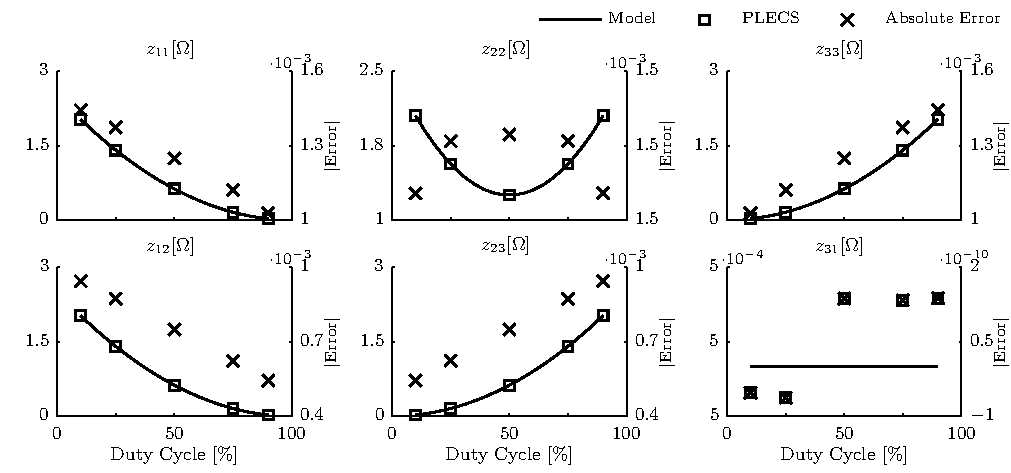
\includegraphics[page=1,width=12cm]{./4_model_validation/APEC_SIM_big}
  \centering
  \caption{SSL comparison between PLECS simulation and the proposed model.}
  \label{fig:sim_ssl}
\end{figure}


\begin{figure}[!h]
  \includegraphics[page=3,width=12cm]{./4_model_validation/APEC_SIM_big}
  \centering
  \caption{FSL comparison between PLECS simulation and the proposed model.}
  \label{fig:sim_fsl}
\end{figure}


\subsection{Experimental results}
An experimental set-up of the converter in was built. The converter uses four MOSFETs TN0104 from Supertex with typical \emph{on}-resistance of 1.5 $\Omega$. Two tantalum electrolytic capacitors of 10$\mu$F have been used as flying capacitors. The circuit was operated at 5kHz and the trans-resistance parameters are measured at different duty cycles. The results are compared with the model and  presented in Figures~\ref{fig:meas_zscc} and~\ref{fig:fsw_Zscc}, it can be seen that the predictions match the measured values with less than 10\% error. All the trans-impedance values with the exception of  parameters $z_{31}$ and $z_{13}$ follow the trend with the duty cycle predicted by the model. $z_{31}$ and $z_{13}$ have a bigger error since these values are much smaller than the rest of the converter parameters and, therefore, more sensitive to the parasitics of the board. In any case, it can be seen that predictive trends, in all presented results, are still consistent for variations in duty cycle and frequency for the model trans-resistance parameters.

\begin{figure}[!h]
\newcommand\pHeigh{2.750cm}
\newcommand\pWidth{2.500cm}
\centering
	\begin{subfigure}{\textwidth}
		\parbox[b]{0.3250\linewidth}{
		\centering
			\begin{tikzpicture}
    \pgfplotsset{
        width=\pWidth,
        height=\pHeigh,
        scale only axis,
        xlabel near ticks,
        ylabel near ticks,
        scaled y ticks= true ,
        enlarge x limits={0.1},
        enlarge y limits={0.1},
        every tick label/.append style={font=\footnotesize},
        }

	\begin{axis}[
		axis y line*=left,
		axis x line*=bottom,
		xticklabels={,,},
		ylabel = {$r_{scc} [\Omega]$},
		yticklabel style={text width=2.00em,align=right},
		title = {$z_{11}$},
		title style = {
    			font=\footnotesize },
    			at ={(0.75,0.75)},
		]

		\addplot[thin,black,smooth]
    		table [y=y1]{./4_model_validation/c10uF_bis/c10uF_bis_5kHz_Ymdl.dat};

		\addplot[semithick,mark=o,only marks]
    		table [y=y1]{./4_model_validation/c10uF_bis/c10uF_bis_5kHz_Ymeas.dat};

\end{axis}

\end{tikzpicture}

		}
		\parbox[b]{0.3250\linewidth}{
		\centering
			\begin{tikzpicture}
    \pgfplotsset{
        width=\pWidth,
        height=\pHeigh,
        scale only axis,
        xlabel near ticks,
        ylabel near ticks,
        scaled y ticks= true ,
        enlarge x limits={0.1},
        enlarge y limits={0.1},
        every tick label/.append style={font=\footnotesize},
        }

	\begin{axis}[
		axis y line*=left,
		axis x line*=bottom,
		xticklabels={,,},
		yticklabel style={text width=1.50em,align=right},
		title = {$z_{12}$},
		title style = {
    			font=\footnotesize },
    			at ={(0.75,0.75)},
		]

		\addplot[thin,black,smooth]
    		table [y=y4]{./4_model_validation/c10uF_bis/c10uF_bis_5kHz_Ymdl.dat};

		\addplot[semithick,mark=square,only marks]
    		table [y=y4]{./4_model_validation/c10uF_bis/c10uF_bis_5kHz_Ymeas.dat};

	\end{axis}

	\begin{axis}[
		axis y line*=right,
		axis x line=none,
		xticklabels={,,},
		yticklabel pos=right,
		yticklabel style={text width=1.50em,align=left,xshift=-0.50ex},
		enlarge y limits={0.15},
		]

		\addplot[semithick,mark=x,only marks]
    		table [y=y4]{./4_model_validation/c10uF_bis/c10uF_bis_5kHz_Yerr.dat};

	\end{axis}

\end{tikzpicture}

		}
		\parbox[b]{0.3250\linewidth}{
		\centering
			\begin{tikzpicture}
    \pgfplotsset{
        width=\pWidth,
        height=\pHeigh,
        scale only axis,
        xlabel near ticks,
        ylabel near ticks,
        scaled y ticks= true ,
        enlarge x limits={0.1},
        enlarge y limits={0.1},
        every tick label/.append style={font=\footnotesize},
        }

	\begin{axis}[
		axis y line*=left,
		axis x line*=bottom,
		xticklabels={,,},
		yticklabel style={text width=2.00em,align=right},
		title = {$z_{13}$},
		title style = {
    			font=\footnotesize },
    			at ={(0.75,0.75)},
		]

		\addplot[thin,black,smooth]
    		table [y=y7]{./4_model_validation/c10uF_bis/c10uF_bis_5kHz_Ymdl.dat};

		\addplot[semithick,mark=o,only marks]
    		table [y=y7]{./4_model_validation/c10uF_bis/c10uF_bis_5kHz_Ymeas.dat};

\end{axis}

\end{tikzpicture}

		}
	\end{subfigure}

	\begin{subfigure}{\textwidth}
		\parbox[b]{0.3250\linewidth}{
		\centering
			\begin{tikzpicture}
    \pgfplotsset{
        width=\pWidth,
        height=\pHeigh,
        scale only axis,
        xlabel near ticks,
        ylabel near ticks,
        scaled y ticks= true ,
        enlarge x limits={0.1},
        enlarge y limits={0.1},
        every tick label/.append style={font=\footnotesize},
        }

	\begin{axis}[
		axis y line*=left,
		axis x line*=bottom,
		xticklabels={,,},
		ylabel = {$r_{scc} [\Omega]$},
		yticklabel style={text width=1.50em,align=right},
		title = {$z_{21}$},
		title style = {
    			font=\footnotesize },
    			at ={(0.75,0.75)},
		]

		\addplot[thin,black,smooth]
    		table [y=y2]{./4_model_validation/c10uF_bis/c10uF_bis_5kHz_Ymdl.dat};

		\addplot[semithick,mark=square,only marks]
    		table [y=y2]{./4_model_validation/c10uF_bis/c10uF_bis_5kHz_Ymeas.dat};

	\end{axis}

	\begin{axis}[
		axis y line*=right,
		axis x line=none,
		xticklabels={,,},
		yticklabel pos=right,
		yticklabel style={text width=1.50em,align=left,xshift=-0.50ex},
		enlarge y limits={0.15},
		]

		\addplot[semithick,mark=x,only marks]
    		table [y=y2]{./4_model_validation/c10uF_bis/c10uF_bis_5kHz_Yerr.dat};

	\end{axis}

\end{tikzpicture}

		}
		\parbox[b]{0.3250\linewidth}{
		\centering
			\begin{tikzpicture}
    \pgfplotsset{
        width=\pWidth,
        height=\pHeigh,
        scale only axis,
        xlabel near ticks,
        ylabel near ticks,
        scaled y ticks= true ,
        enlarge x limits={0.1},
        enlarge y limits={0.1},
        every tick label/.append style={font=\footnotesize},
        }

	\begin{axis}[
		axis y line*=left,
		axis x line*=bottom,
		xticklabels={,,},
		yticklabel style={text width=2.00em,align=right},
		title = {$z_{22}$},
		title style = {
    			font=\footnotesize },
    			at ={(0.75,0.75)},
		]

		\addplot[thin,black,smooth]
    		table [y=y5]{./4_model_validation/c10uF_bis/c10uF_bis_5kHz_Ymdl.dat};

		\addplot[semithick,mark=o,only marks]
    		table [y=y5]{./4_model_validation/c10uF_bis/c10uF_bis_5kHz_Ymeas.dat};

\end{axis}

\end{tikzpicture}

		}
		\parbox[b]{0.3250\linewidth}{
		\centering
			\begin{tikzpicture}
    \pgfplotsset{
        width=\pWidth,
        height=\pHeigh,
        scale only axis,
        xlabel near ticks,
        ylabel near ticks,
        scaled y ticks= true ,
        enlarge x limits={0.1},
        enlarge y limits={0.1},
        every tick label/.append style={font=\footnotesize},
        }

	\begin{axis}[
		axis y line*=left,
		axis x line*=bottom,
		xticklabels={,,},
		yticklabel style={text width=1.50em,align=right},
		title = {$z_{23}$},
		title style = {
    			font=\footnotesize },
    			at ={(0.75,0.75)},
		]

		\addplot[thin,black,smooth]
    		table [y=y8]{./4_model_validation/c10uF_bis/c10uF_bis_5kHz_Ymdl.dat};

		\addplot[semithick,mark=square,only marks]
    		table [y=y8]{./4_model_validation/c10uF_bis/c10uF_bis_5kHz_Ymeas.dat};

	\end{axis}

	\begin{axis}[
		axis y line*=right,
		axis x line=none,
		xticklabels={,,},
		ylabel = {$\epsilon$},
		yticklabel pos=right,
		yticklabel style={text width=1.50em,align=left,xshift=-0.50ex},
		enlarge y limits={0.15},
		]

		\addplot[semithick,mark=x,only marks]
    		table [y=y8]{./4_model_validation/c10uF_bis/c10uF_bis_5kHz_Yerr.dat};

	\end{axis}

\end{tikzpicture}

		}
	\end{subfigure}

	\begin{subfigure}{\textwidth}
		\parbox[b]{0.3250\linewidth}{
		\centering
			\begin{tikzpicture}
    \pgfplotsset{
        width=\pWidth,
        height=\pHeigh,
        scale only axis,
        xlabel near ticks,
        ylabel near ticks,
        scaled y ticks= true ,
        enlarge x limits={0.1},
        enlarge y limits={0.1},
        every tick label/.append style={font=\footnotesize},
        }

	\begin{axis}[
		axis y line*=left,
		axis x line*=bottom,
		xlabel = {duty cycle},
		ylabel = {$r_{scc} [\Omega]$},
		yticklabel style={text width=1.50em,align=right},
		title = {$z_{31}$},
		title style = {
    			font=\footnotesize },
    			at ={(0.75,0.75)},
		]

		\addplot[thin,black,smooth]
    		table [y=y3]{./4_model_validation/c10uF_bis/c10uF_bis_5kHz_Ymdl.dat};

		\addplot[semithick,mark=square,only marks]
    		table [y=y3]{./4_model_validation/c10uF_bis/c10uF_bis_5kHz_Ymeas.dat};

	\end{axis}

	\begin{axis}[
		axis y line*=right,
		axis x line=none,
		yticklabel pos=right,
		yticklabel style={text width=1.50em,align=left,xshift=-0.50ex},
		enlarge y limits={0.15},
		]

		\addplot[semithick,mark=x,only marks]
    		table [y=y3]{./4_model_validation/c10uF_bis/c10uF_bis_5kHz_Yerr.dat};

	\end{axis}

\end{tikzpicture}

		}
		\parbox[b]{0.3250\linewidth}{
		\centering
			\begin{tikzpicture}
    \pgfplotsset{
        width=\pWidth,
        height=\pHeigh,
        scale only axis,
        xlabel near ticks,
        ylabel near ticks,
        scaled y ticks= true ,
        enlarge x limits={0.1},
        enlarge y limits={0.1},
        every tick label/.append style={font=\footnotesize},
        }

	\begin{axis}[
		axis y line*=left,
		axis x line*=bottom,
		xlabel = {duty cycle},
		yticklabel style={text width=1.50em,align=right},
		title = {$z_{32}$},
		title style = {
    			font=\footnotesize },
    			at ={(0.75,0.75)},
		]

		\addplot[thin,black,smooth]
    		table [y=y6]{./4_model_validation/c10uF_bis/c10uF_bis_5kHz_Ymdl.dat};

		\addplot[semithick,mark=square,only marks]
    		table [y=y6]{./4_model_validation/c10uF_bis/c10uF_bis_5kHz_Ymeas.dat};

	\end{axis}

	\begin{axis}[
		axis y line*=right,
		axis x line=none,
		yticklabel pos=right,
		yticklabel style={text width=1.50em,align=left,xshift=-0.50ex},
		enlarge y limits={0.15},
		]

		\addplot[semithick,mark=x,only marks]
    		table [y=y6]{./4_model_validation/c10uF_bis/c10uF_bis_5kHz_Yerr.dat};

	\end{axis}

\end{tikzpicture}

		}
		\parbox[b]{0.3250\linewidth}{
		\centering
			\begin{tikzpicture}
    \pgfplotsset{
        width=\pWidth,
        height=\pHeigh,
        scale only axis,
        xlabel near ticks,
        ylabel near ticks,
        scaled y ticks= true ,
        enlarge x limits={0.1},
        enlarge y limits={0.1},
        every tick label/.append style={font=\footnotesize},
        }

	\begin{axis}[
		axis y line*=left,
		axis x line*=bottom,
		xlabel = {duty cycle},
		yticklabel style={text width=2.00em,align=right},
		title = {$z_{33}$},
		title style = {
    			font=\footnotesize },
    			at ={(0.75,0.75)},
		]

		\addplot[thin,black,smooth]
    		table [y=y9]{./4_model_validation/c10uF_bis/c10uF_bis_5kHz_Ymdl.dat};

		\addplot[semithick,mark=o,only marks]
    		table [y=y9]{./4_model_validation/c10uF_bis/c10uF_bis_5kHz_Ymeas.dat};

\end{axis}

\end{tikzpicture}

		}
	\end{subfigure}

	\caption[Measured $\mathbf{Z_{scc}}$ from a 2:1 SCC experimental converter.]{Experimental results of the 2:1 SCC, with $f_{sw}=5kHz$. Comparison of the  measured (\emph{$\Box$ markers} ) trans-resistance parameters with the model predicted (\emph{solid line}), and the error ($\epsilon$) between the model and the measures (\emph{x markers}.)}
	\label{}
\end{figure}



\begin{figure}[!h]
\newcommand\pHeigh{2.750cm}
\newcommand\pWidth{2.500cm}
\centering
	\begin{subfigure}{\textwidth}
		\parbox[b]{0.3250\linewidth}{
		\centering
			\begin{tikzpicture}
    \pgfplotsset{
        width=\pWidth,
        height=\pHeigh,
        scale only axis,
        xlabel near ticks,
        ylabel near ticks,
        scaled y ticks= true ,
        enlarge x limits={0.1},
        enlarge y limits={0.1},
        every tick label/.append style={font=\footnotesize},
        }

	\begin{loglogaxis}[
		axis y line*=left,
		axis x line*=bottom,
		xticklabels={,,},
		ylabel = {$[\Omega]$},
		yticklabel style={text width=2.00em,align=right},
		title = {$z_{11}$},
		title style = {
    			font=\footnotesize },
    			at ={(0.75,0.75)},
		]

		\addplot[thin,black,smooth]
    		table [y=y1]{./4_model_validation/c10uF_bis_fsw/c10uF_bis_fsw_D=50_Ymdl.dat};

		\addplot[semithick,mark=square,only marks]
    		table [y=y1]{./4_model_validation/c10uF_bis_fsw/c10uF_bis_fsw_D=50_Ymeas.dat};

	\end{loglogaxis}

\end{tikzpicture}

		}
		\parbox[b]{0.3250\linewidth}{
		\centering
			\begin{tikzpicture}
    \pgfplotsset{
        width=\pWidth,
        height=\pHeigh,
        scale only axis,
        xlabel near ticks,
        ylabel near ticks,
        scaled y ticks= true ,
        enlarge x limits={0.1},
        enlarge y limits={0.1},
        every tick label/.append style={font=\footnotesize},
        }

	\begin{loglogaxis}[
		axis y line*=left,
		axis x line*=bottom,
		xticklabels={,,},
		yticklabel style={text width=2.00em,align=right},
		title = {$z_{12}$},
		title style = {
    			font=\footnotesize },
    			at ={(0.75,0.75)},
		]

		\addplot[thin,black,smooth]
    		table [y=y4]{./4_model_validation/c10uF_bis_fsw/c10uF_bis_fsw_D=50_Ymdl.dat};

		\addplot[semithick,mark=square,only marks]
    		table [y=y4]{./4_model_validation/c10uF_bis_fsw/c10uF_bis_fsw_D=50_Ymeas.dat};

	\end{loglogaxis}

\end{tikzpicture}

		}
		\parbox[b]{0.3250\linewidth}{
		\centering
			\begin{tikzpicture}
    \pgfplotsset{
        width=\pWidth,
        height=\pHeigh,
        scale only axis,
        xlabel near ticks,
        ylabel near ticks,
        scaled y ticks= true ,
        enlarge x limits={0.1},
        enlarge y limits={0.1},
        every tick label/.append style={font=\footnotesize},
        }

	\begin{loglogaxis}[
		axis y line*=left,
		axis x line*=bottom,
		xticklabels={,,},
		yticklabel style={text width=2.00em,align=right},
		title = {$z_{13}$},
		title style = {
    			font=\footnotesize },
    			at ={(0.75,0.75)},
		]

		\addplot[thin,black,smooth]
    		table [y=y7]{./4_model_validation/c10uF_bis_fsw/c10uF_bis_fsw_D=50_Ymdl.dat};

		\addplot[semithick,mark=square,only marks]
    		table [y=y7]{./4_model_validation/c10uF_bis_fsw/c10uF_bis_fsw_D=50_Ymeas.dat};

	\end{loglogaxis}

\end{tikzpicture}

		}
	\end{subfigure}

	\begin{subfigure}{\textwidth}
		\parbox[b]{0.3250\linewidth}{
		\centering
			\begin{tikzpicture}
    \pgfplotsset{
        width=\pWidth,
        height=\pHeigh,
        scale only axis,
        xlabel near ticks,
        ylabel near ticks,
        scaled y ticks= true ,
        enlarge x limits={0.1},
        enlarge y limits={0.1},
        every tick label/.append style={font=\footnotesize},
        }

	\begin{loglogaxis}[
		axis y line*=left,
		axis x line*=bottom,
		xticklabels={,,},
		ylabel = {$[\Omega]$},
		yticklabel style={text width=2.00em,align=right},
		title = {$z_{21}$},
		title style = {
    			font=\footnotesize },
    			at ={(0.75,0.75)},
		]

		\addplot[thin,black,smooth]
    		table [y=y2]{./4_model_validation/c10uF_bis_fsw/c10uF_bis_fsw_D=50_Ymdl.dat};

		\addplot[semithick,mark=square,only marks]
    		table [y=y2]{./4_model_validation/c10uF_bis_fsw/c10uF_bis_fsw_D=50_Ymeas.dat};

	\end{loglogaxis}

\end{tikzpicture}

		}
		\parbox[b]{0.3250\linewidth}{
		\centering
			\begin{tikzpicture}
    \pgfplotsset{
        width=\pWidth,
        height=\pHeigh,
        scale only axis,
        xlabel near ticks,
        ylabel near ticks,
        scaled y ticks= true ,
        enlarge x limits={0.1},
        enlarge y limits={0.1},
        every tick label/.append style={font=\footnotesize},
        }

	\begin{loglogaxis}[
		axis y line*=left,
		axis x line*=bottom,
		xticklabels={,,},
		yticklabel style={text width=2.00em,align=right},
		title = {$z_{22}$},
		title style = {
    			font=\footnotesize },
    			at ={(0.75,0.75)},
		]

		\addplot[thin,black,smooth]
    		table [y=y5]{./4_model_validation/c10uF_bis_fsw/c10uF_bis_fsw_D=50_Ymdl.dat};

		\addplot[semithick,mark=square,only marks]
    		table [y=y5]{./4_model_validation/c10uF_bis_fsw/c10uF_bis_fsw_D=50_Ymeas.dat};

	\end{loglogaxis}

\end{tikzpicture}

		}
		\parbox[b]{0.3250\linewidth}{
		\centering
			\begin{tikzpicture}
    \pgfplotsset{
        width=\pWidth,
        height=\pHeigh,
        scale only axis,
        xlabel near ticks,
        ylabel near ticks,
        scaled y ticks= true ,
        enlarge x limits={0.1},
        enlarge y limits={0.1},
        every tick label/.append style={font=\footnotesize},
        }

	\begin{loglogaxis}[
		axis y line*=left,
		axis x line*=bottom,
		xticklabels={,,},
		yticklabel style={text width=2.00em,align=right},
		title = {$z_{23}$},
		title style = {
    			font=\footnotesize },
    			at ={(0.75,0.75)},
		]

		\addplot[thin,black,smooth]
    		table [y=y8]{./4_model_validation/c10uF_bis_fsw/c10uF_bis_fsw_D=50_Ymdl.dat};

		\addplot[semithick,mark=square,only marks]
    		table [y=y8]{./4_model_validation/c10uF_bis_fsw/c10uF_bis_fsw_D=50_Ymeas.dat};

	\end{loglogaxis}

\end{tikzpicture}

		}
	\end{subfigure}

	\begin{subfigure}{\textwidth}
		\parbox[b]{0.3250\linewidth}{
		\centering
			\begin{tikzpicture}
    \pgfplotsset{
        width=\pWidth,
        height=\pHeigh,
        scale only axis,
        xlabel near ticks,
        ylabel near ticks,
        scaled y ticks= true ,
        enlarge x limits={0.1},
        enlarge y limits={0.1},
        every tick label/.append style={font=\footnotesize},
        }

	\begin{loglogaxis}[
		axis y line*=left,
		axis x line*=bottom,
		xlabel = {$f_{sw}$},
		ylabel = {$[\Omega]$},
		yticklabel style={text width=2.00em,align=right},
		title = {$z_{31}$},
		title style = {
    			font=\footnotesize },
    			at ={(0.75,0.75)},
		]

		\addplot[thin,black,smooth]
    		table [y=y3]{./4_model_validation/c10uF_bis_fsw/c10uF_bis_fsw_D=50_Ymdl.dat};

		\addplot[semithick,mark=square,only marks]
    		table [y=y3]{./4_model_validation/c10uF_bis_fsw/c10uF_bis_fsw_D=50_Ymeas.dat};

	\end{loglogaxis}

\end{tikzpicture}

		}
		\parbox[b]{0.3250\linewidth}{
		\centering
			\begin{tikzpicture}
    \pgfplotsset{
        width=\pWidth,
        height=\pHeigh,
        scale only axis,
        xlabel near ticks,
        ylabel near ticks,
        scaled y ticks= true ,
        enlarge x limits={0.1},
        enlarge y limits={0.1},
        every tick label/.append style={font=\footnotesize},
        }

	\begin{loglogaxis}[
		axis y line*=left,
		axis x line*=bottom,
		xlabel = {$f_{sw}$},
		yticklabel style={text width=2.00em,align=right},
		title = {$z_{32}$},
		title style = {
    			font=\footnotesize },
    			at ={(0.75,0.75)},
		]

		\addplot[thin,black,smooth]
    		table [y=y6]{./4_model_validation/c10uF_bis_fsw/c10uF_bis_fsw_D=50_Ymdl.dat};

		\addplot[semithick,mark=square,only marks]
    		table [y=y6]{./4_model_validation/c10uF_bis_fsw/c10uF_bis_fsw_D=50_Ymeas.dat};

	\end{loglogaxis}

\end{tikzpicture}

		}
		\parbox[b]{0.3250\linewidth}{
		\centering
			\begin{tikzpicture}
    \pgfplotsset{
        width=\pWidth,
        height=\pHeigh,
        scale only axis,
        xlabel near ticks,
        ylabel near ticks,
        scaled y ticks= true ,
        enlarge x limits={0.1},
        enlarge y limits={0.1},
        every tick label/.append style={font=\footnotesize},
        }

	\begin{loglogaxis}[
		axis y line*=left,
		axis x line*=bottom,
		xlabel = {$f_{sw}$},
		yticklabel style={text width=2.00em,align=right},
		title = {$z_{33}$},
		title style = {
    			font=\footnotesize },
    			at ={(0.75,0.75)},
		]

		\addplot[thin,black,smooth]
    		table [y=y9]{./4_model_validation/c10uF_bis_fsw/c10uF_bis_fsw_D=50_Ymdl.dat};

		\addplot[semithick,mark=square,only marks]
    		table [y=y9]{./4_model_validation/c10uF_bis_fsw/c10uF_bis_fsw_D=50_Ymeas.dat};

	\end{loglogaxis}

\end{tikzpicture}

		}
	\end{subfigure}

	\caption[Measured $\mathbf{Z_{scc}}$ from a 2:1 SCC experimental converter.]{Experimental results of the 2:1 SCC, with $f_{sw}=50Hz$. Comparison of the  measured (\emph{$\Box$ markers} ) trans-resistance parameters with the model predicted (\emph{solid line}), and the error ($\epsilon$) between the model and the measures (\emph{x markers}.)}
	\label{}
\end{figure}



%The measured results of the experimental set-up can be improved mounting the circuit in a PCB with less parasitics and operated at higher switching frequencies by using ceramic capacitors instead of the tantalum ones .
\section{Summary}
The presented model is a valuable tool for  modeling a broad range of SCCs, from the classical approach of a single output converter to the new architectures where SCCs are combined with inductors. Unlike the previous models, this method allows to model the behaviour of multiple current loaded outputs, including their coupling relations. The model has been verified with simulations and experiments, and for both cases compares favorably. Since the resulting model is based on analytical expressions; the computation time is dramatically faster than any time-domain based simulator.

At the same time, it has been demonstrated that the original charge flow method was inaccurate in the SSL region, specially when the output capacitor was comparable in size to the flying capacitors. And it was not sensible to the variations of the duty cycle, leading to the wrong estimation of the output resistance of the converter.

The results presented the best accuracy of the model when the converter operates close to the well-defined switching limits, SSL and FSL, with relative errors below $5\%$. When the converter operates in region between the two limits, the relative error can increase up to $20\%$, since the value is approximated from the two asymptotical limits. With regard to the different proposed approximations, results shown the best accuracy using the first proposed approximation of $r_{scc} = \sqrt{r_{ssl}^2 + r_{fsl}^2}$.

\clearpage
\bibliographystyle{plainnat}
\bibliography{references} 